\begin{frame}
	\centering
	\begin{tikzpicture}
		\path[use as bounding box] (-6,0) -- (2,0);
		\node at (0,0) {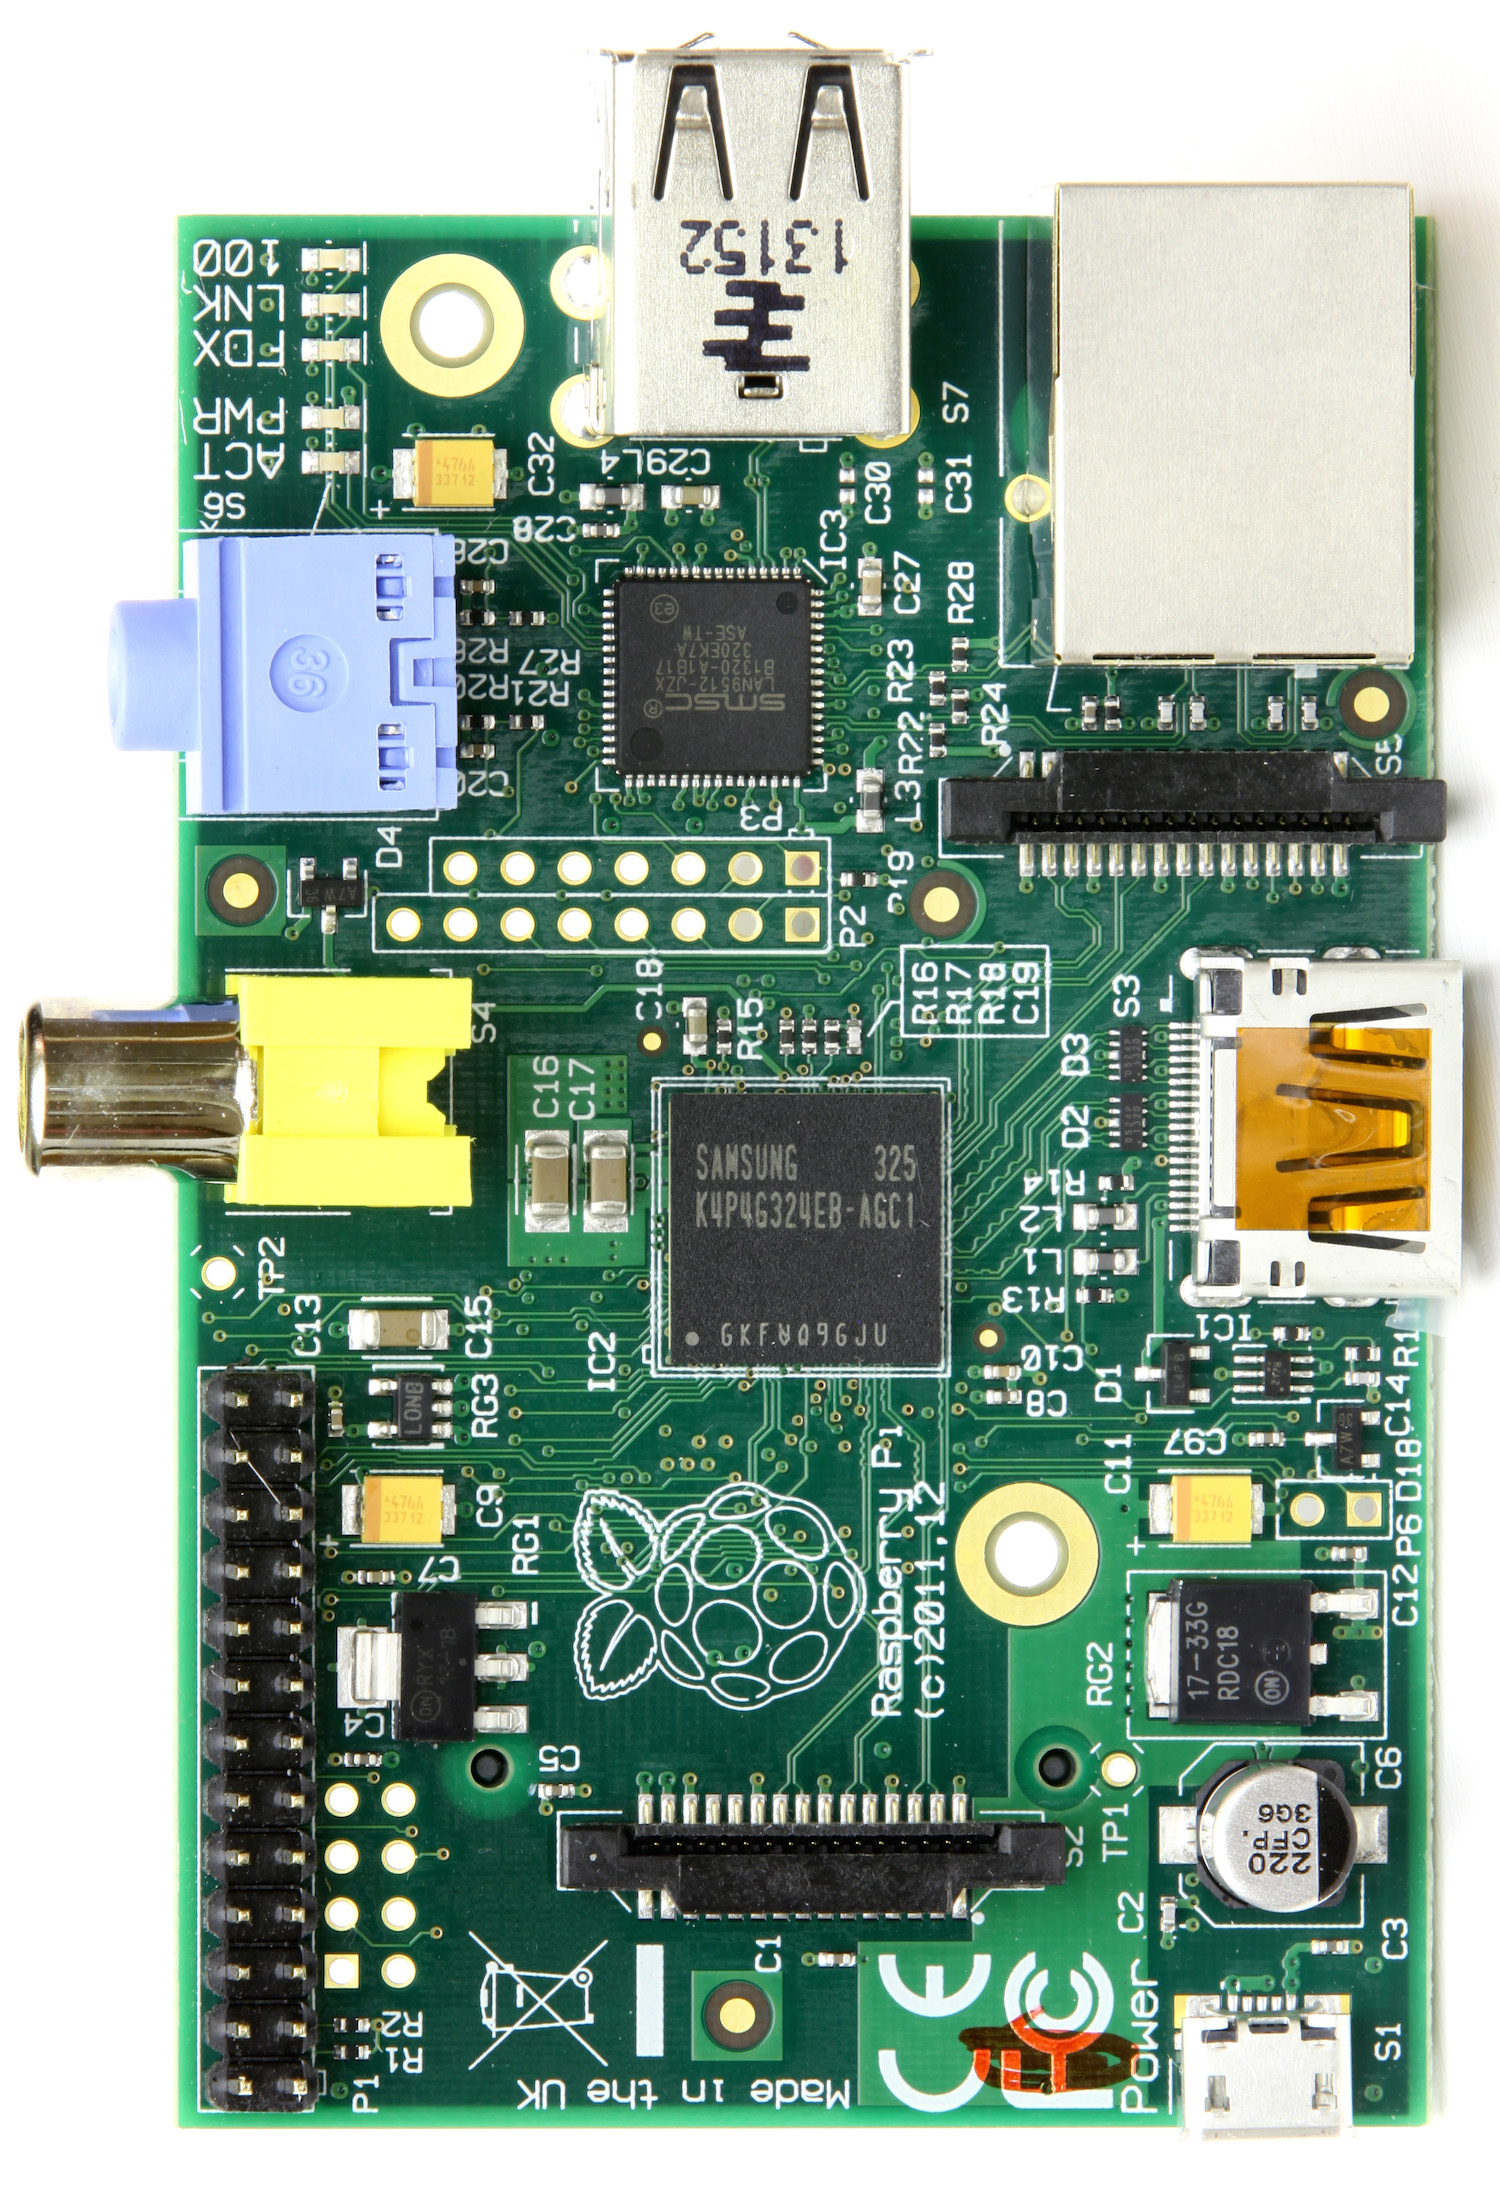
\includegraphics[width=3cm]{img/raspi.jpg}};
		\pause
		\node at (-2.8,-2.1) {
\includegraphics[width=4cm]{img/music.png}};
		\pause
		\path[snake=expanding waves,segment length=2mm,segment angle=30,draw,thick,color=blue] (-1.3,0.85) -- +(-2,0);
	\end{tikzpicture}
\end{frame}

\begin{frame}
    \centering
    \begin{tikzpicture}
		\path[use as bounding box] (-6,0) -- (2,0);
      \node at (0,0) {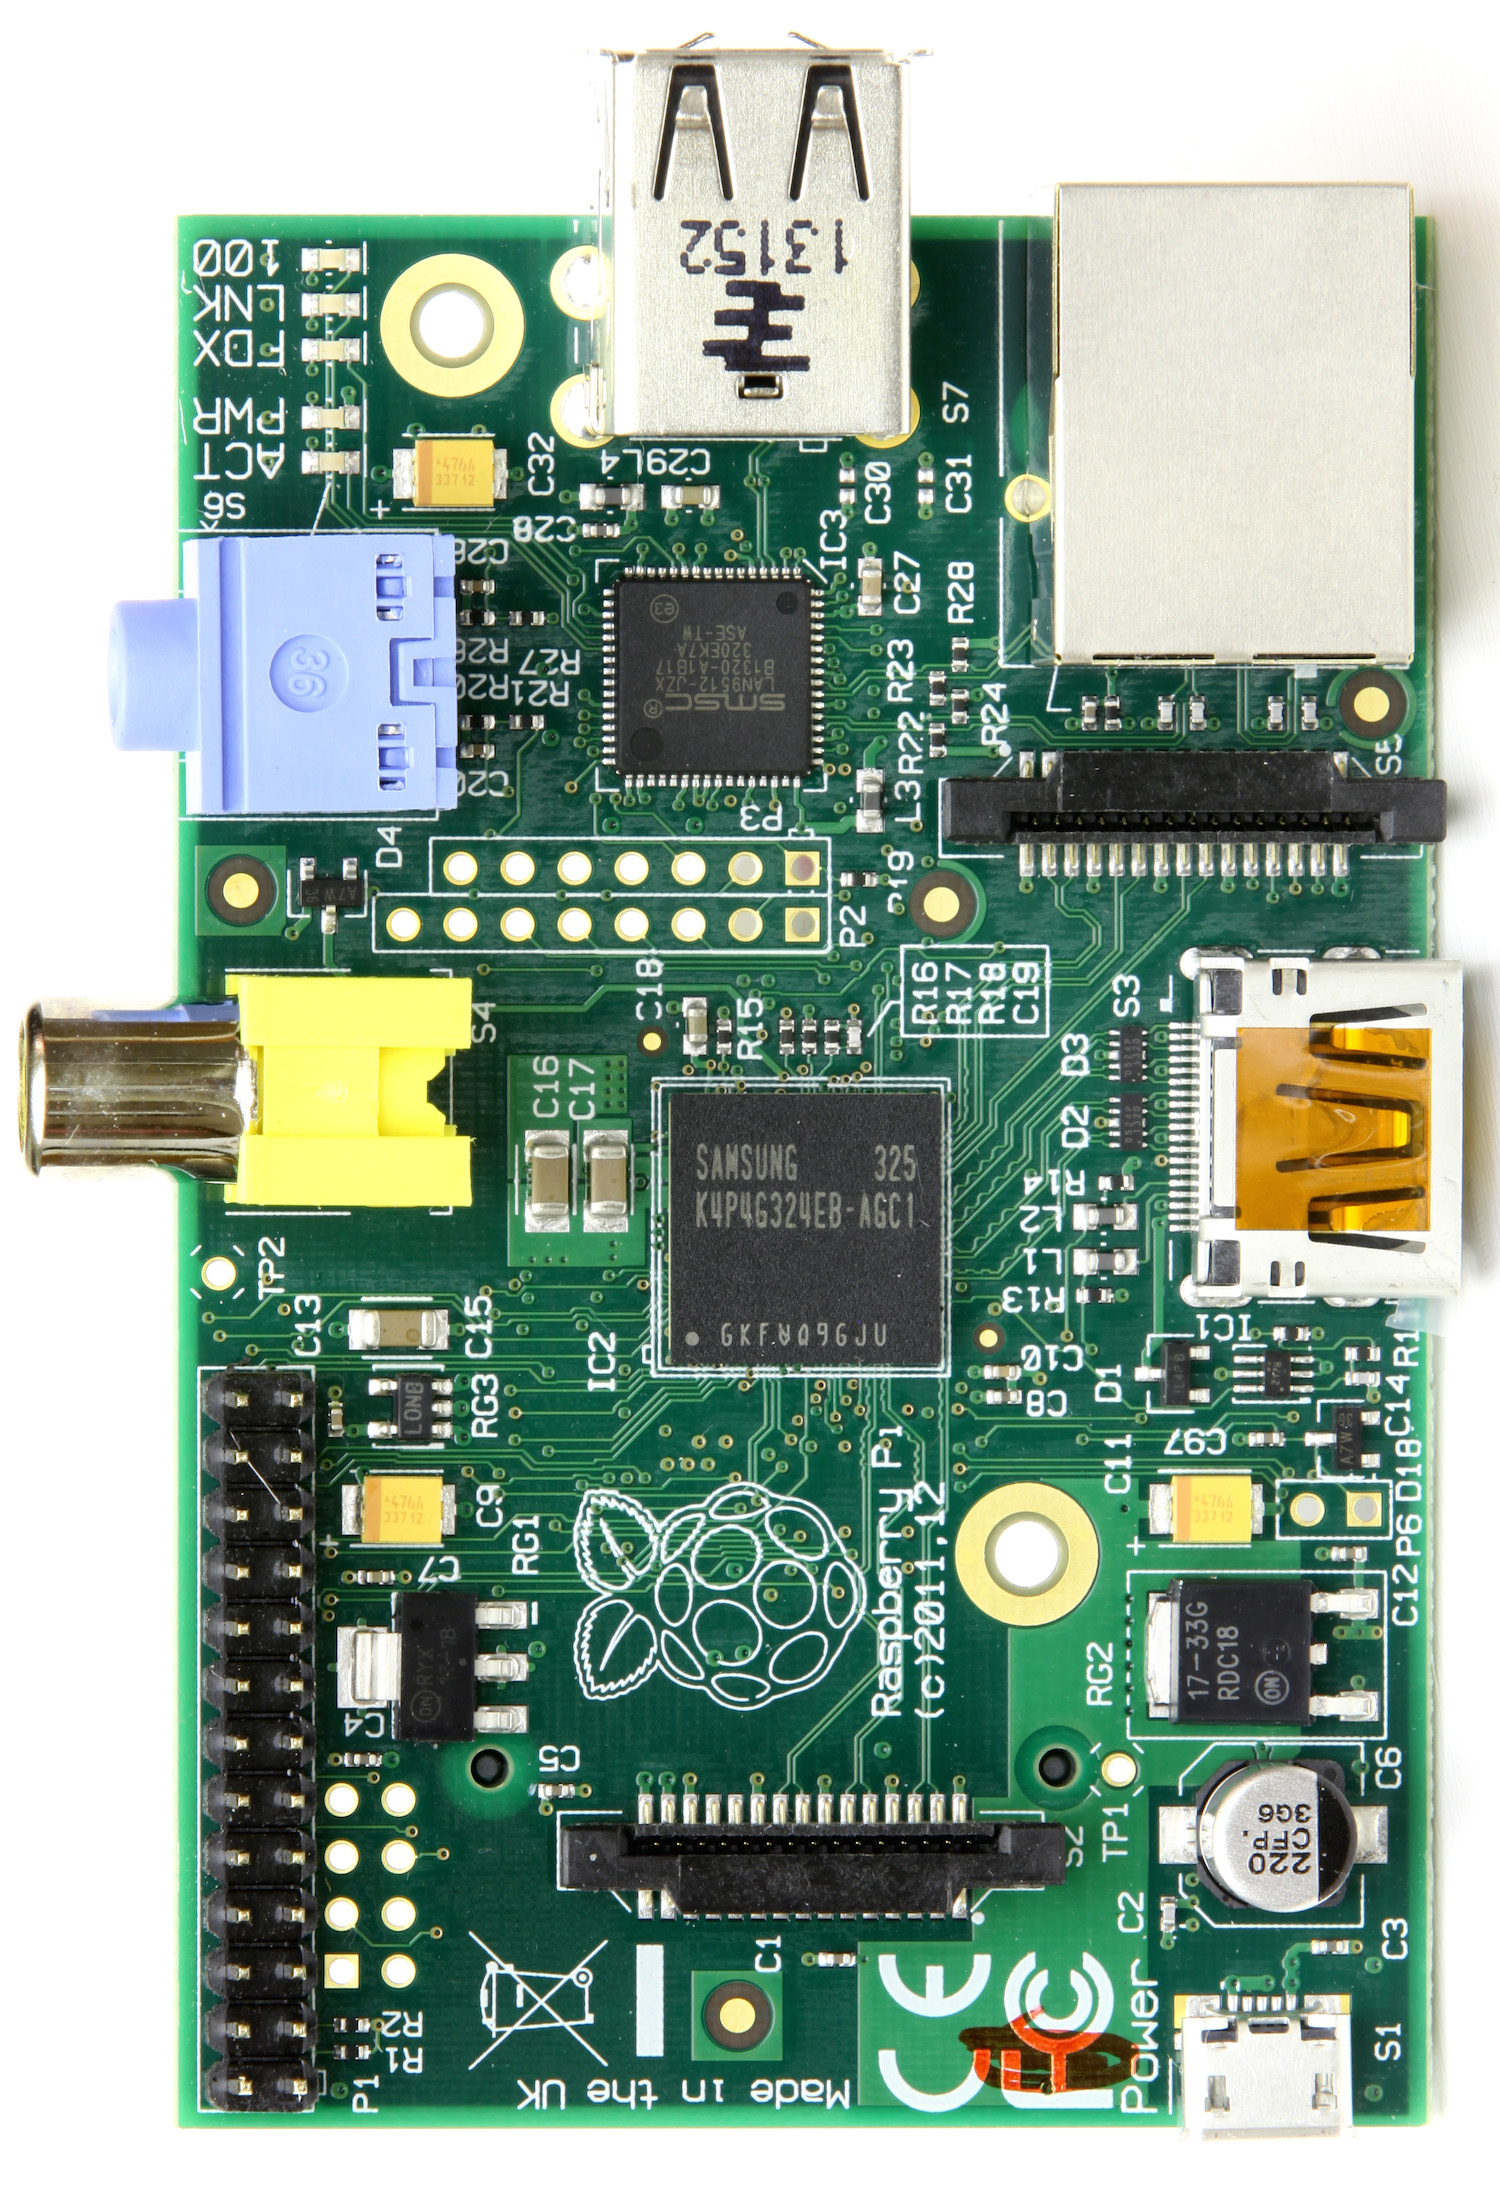
\includegraphics[width=3cm]{img/raspi.jpg}};
      \path[snake=expanding waves,segment length=2mm,segment angle=30,draw,thick,color=blue] (-1.3,0.85) -- +(-2,0);
      %\draw[ultra thick] plot [smooth,tension=1.5] coordinates{(-1,-1) (-2.2, -1.6) (-4, -1.2) (-4.5, -3)};
	  \draw[ultra thick] (-0.95,-1.1) .. controls(-1.5,-3) and (-4,0) .. (-4.5,-3);
      \node at (-4.5, -3) {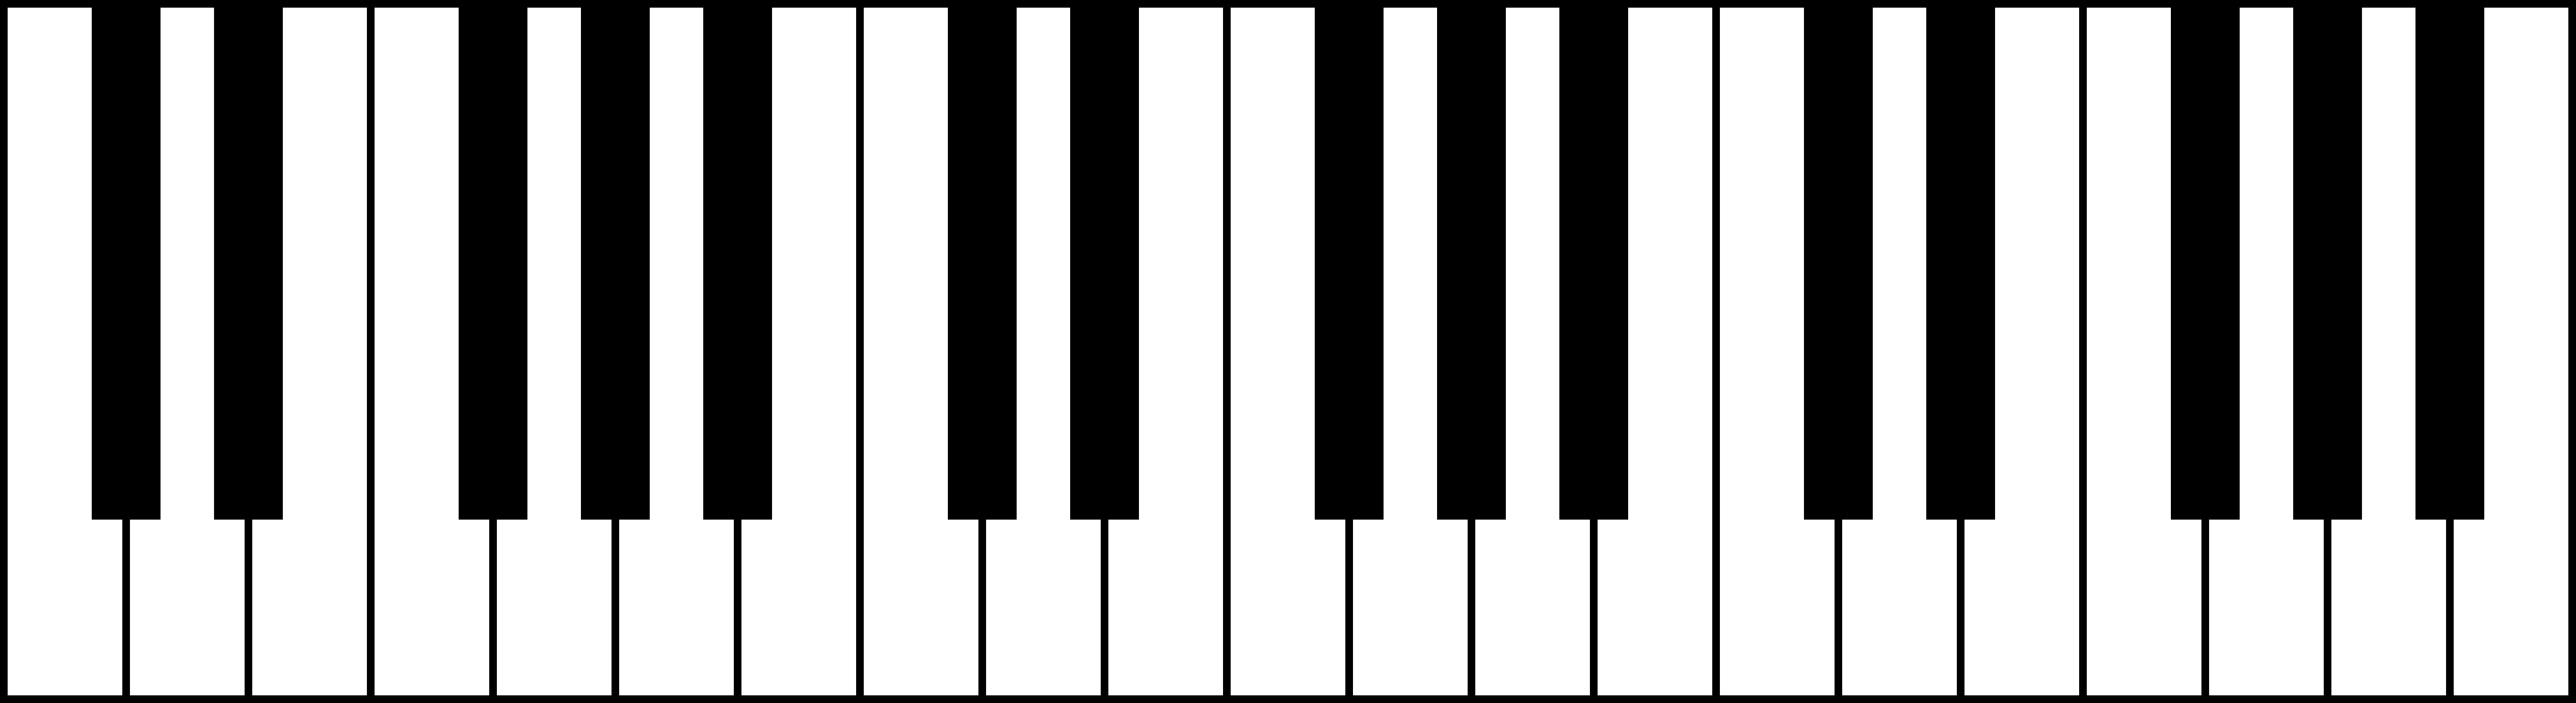
\includegraphics[width=5cm]{img/Musical_keyboard.png}};
    \end{tikzpicture}
\end{frame}

\begin{frame}
	\centering
	\begin{tikzpicture}
		%\path[use as bounding box] (-6,0) -- (2,0);
		\node at (0,0) {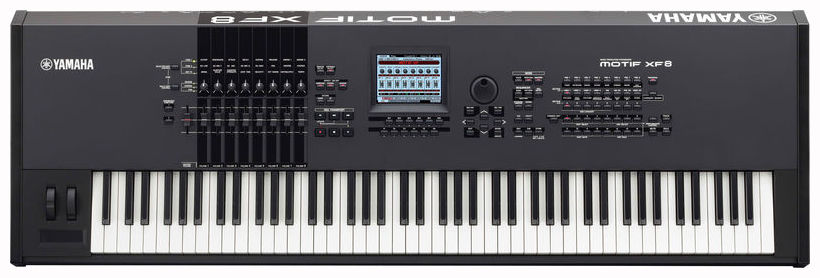
\includegraphics[width=10cm]{img/yamaha.jpg}};
	\end{tikzpicture}
\end{frame}

\begin{frame}
	\centering
	\begin{tikzpicture}
		%\path[use as bounding box] (-6,0) -- (2,0);
		\node at (0,0) {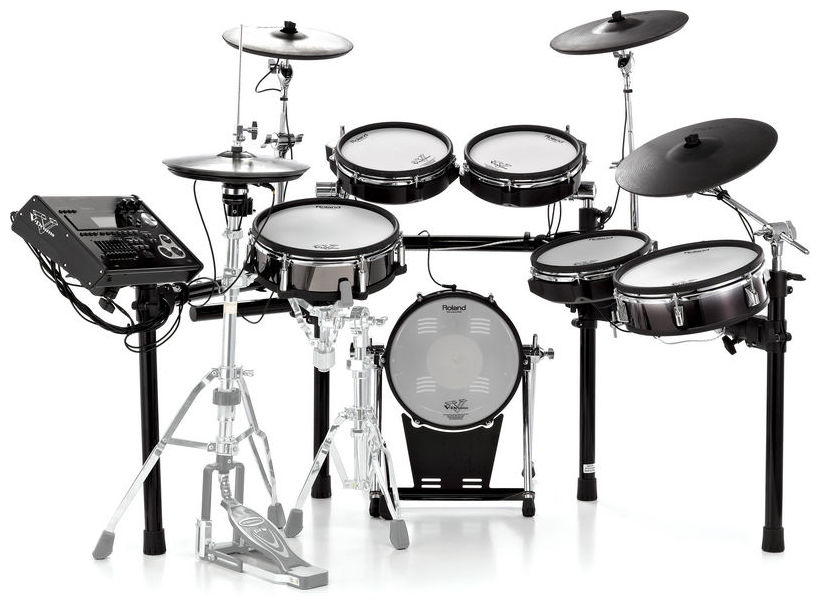
\includegraphics[width=10cm]{img/roland.jpg}};
	\end{tikzpicture}
\end{frame}

\begin{frame}
	\frametitle{GPIO Keyboard}
	\centering
	\begin{tikzpicture}
		\node at (-4,2) {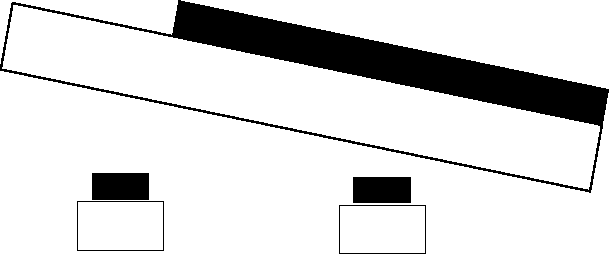
\includegraphics[width=4cm]{img/key1.pdf}};
		\node[align=left ,text width=4cm] at (1,2) { Two buttons connected \\ to GPIO ports};
		\node at (-4,0) {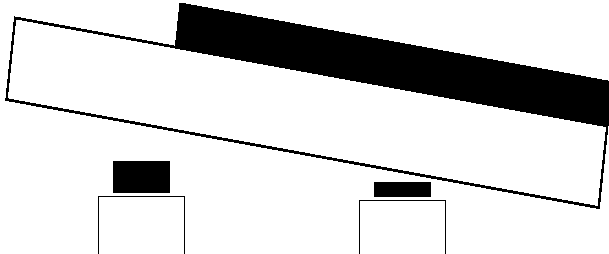
\includegraphics[width=4cm ]{img/key2.pdf}};
		\node[align=left ,text width=4cm] at (1,0) { Interrupt Time A};
		\node at (-4,-2) {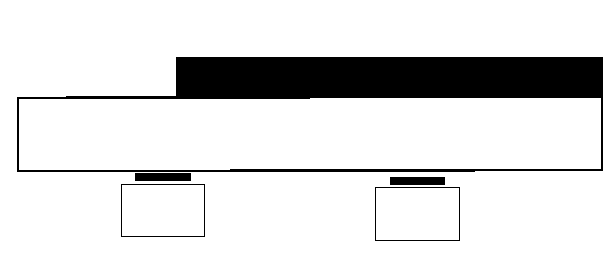
\includegraphics[width=4cm]{img/key3.pdf}};
		\node[align=left ,text width=4cm] at (1,-2) { Interrupt Time B};
		\node[align=left ,text width=6cm] at (-1,-3.5) {  $midi\_velocity=\frac{idle\_stroke}{Time B - Time A}$};
	\end{tikzpicture}	
	
\end{frame}


{
    \usebackgroundtemplate{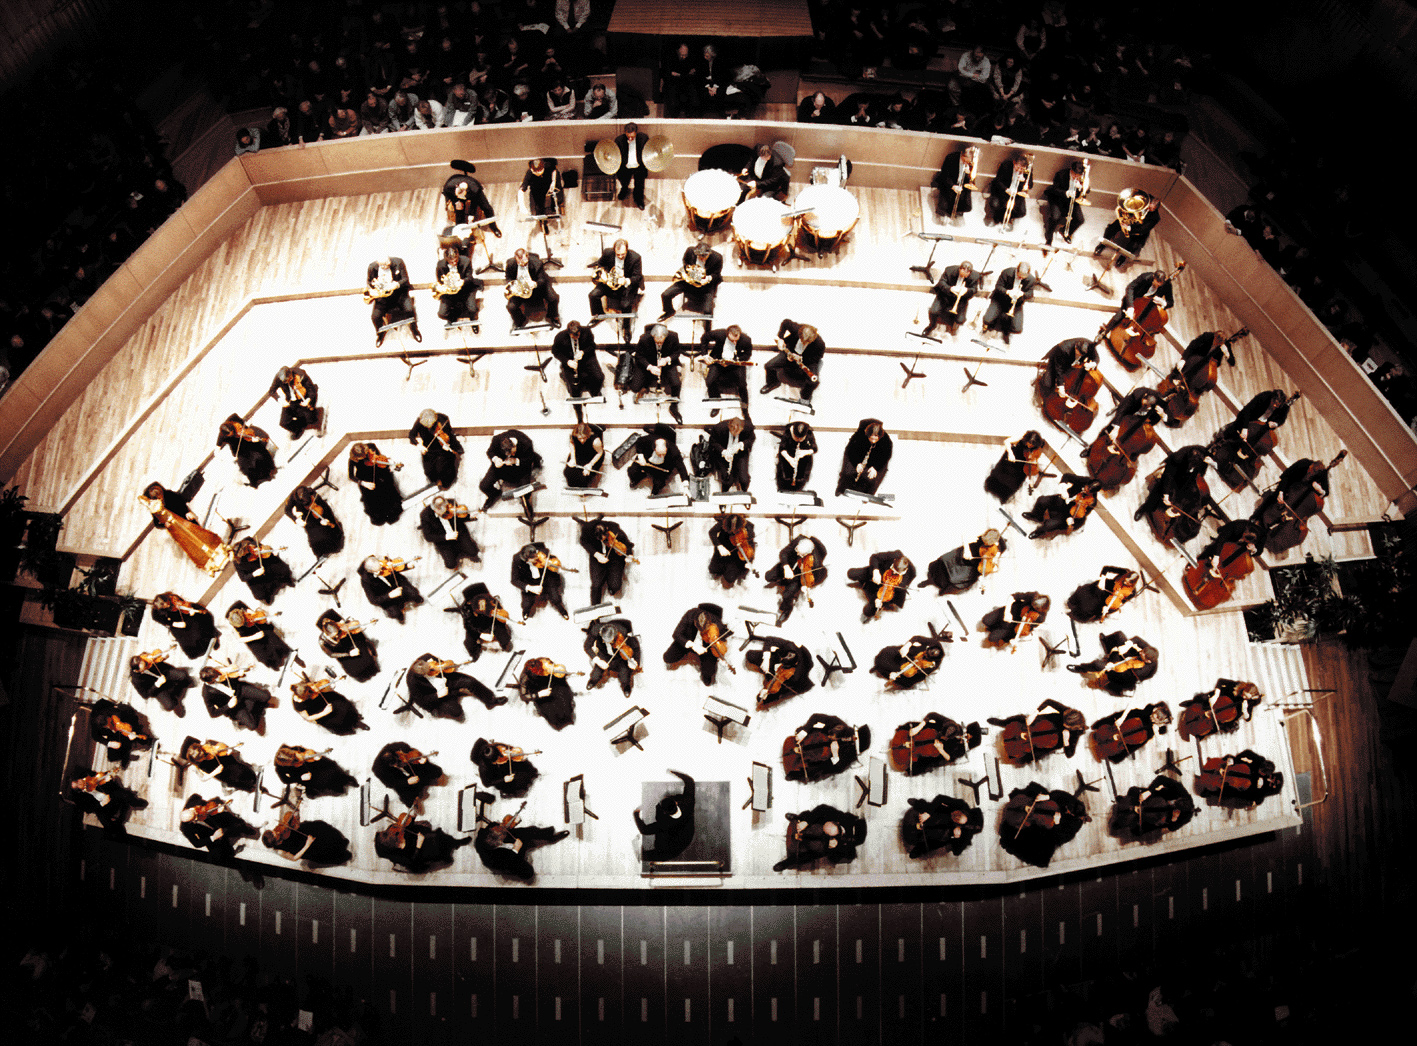
\includegraphics[height=\paperheight]{img/orchestra.jpg}}
    \setbeamertemplate{navigation symbols}{}
    \begin{frame}[plain]
    \end{frame}
}
{
    \usebackgroundtemplate{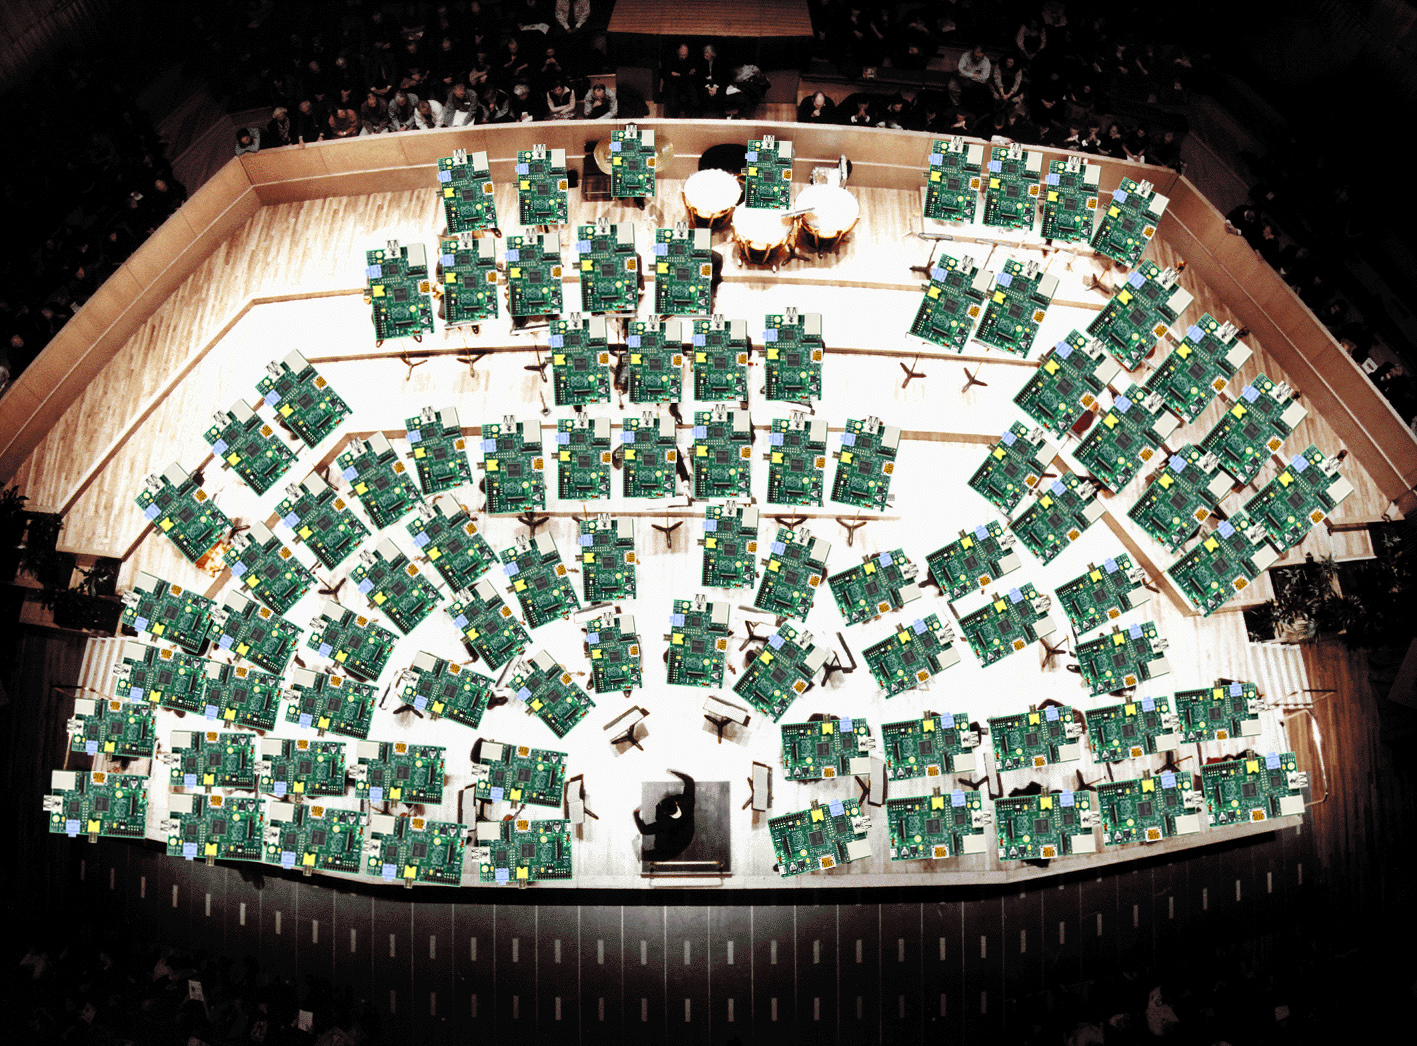
\includegraphics[height=\paperheight]{img/piorchestra.jpg}}
    \setbeamertemplate{navigation symbols}{}
    \begin{frame}[plain]
    \end{frame}
}
\begin{frame}{Composer}
	\centering
	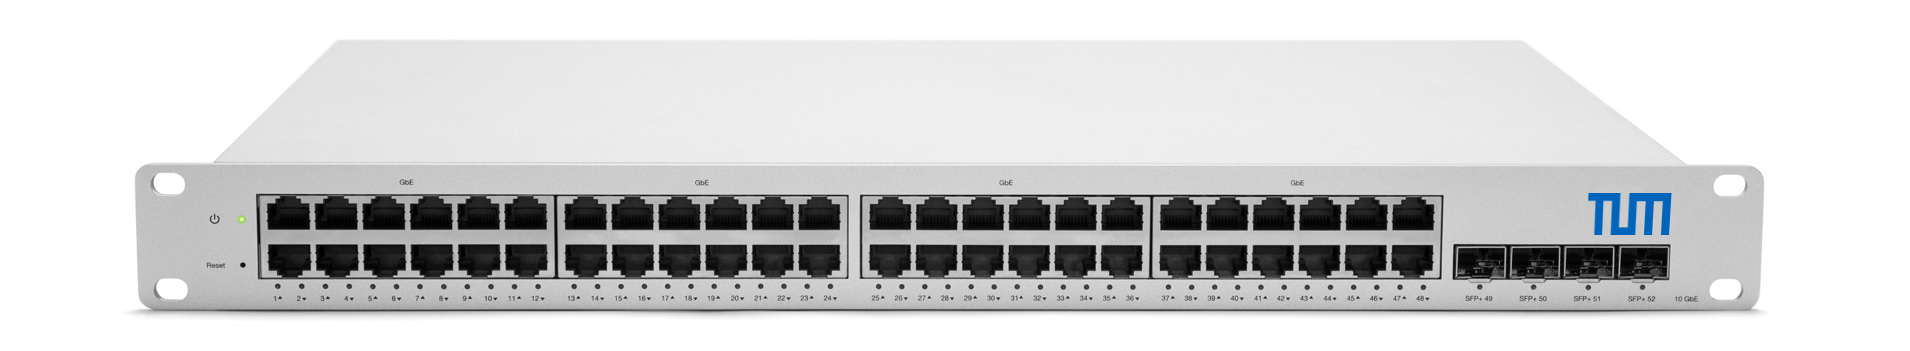
\includegraphics[width=10cm]{img/switch-raw.jpg}
\end{frame}

%\begin{frame}
%	\centering
%	\begin{tikzpicture}
%		\node at (0,-1.2) {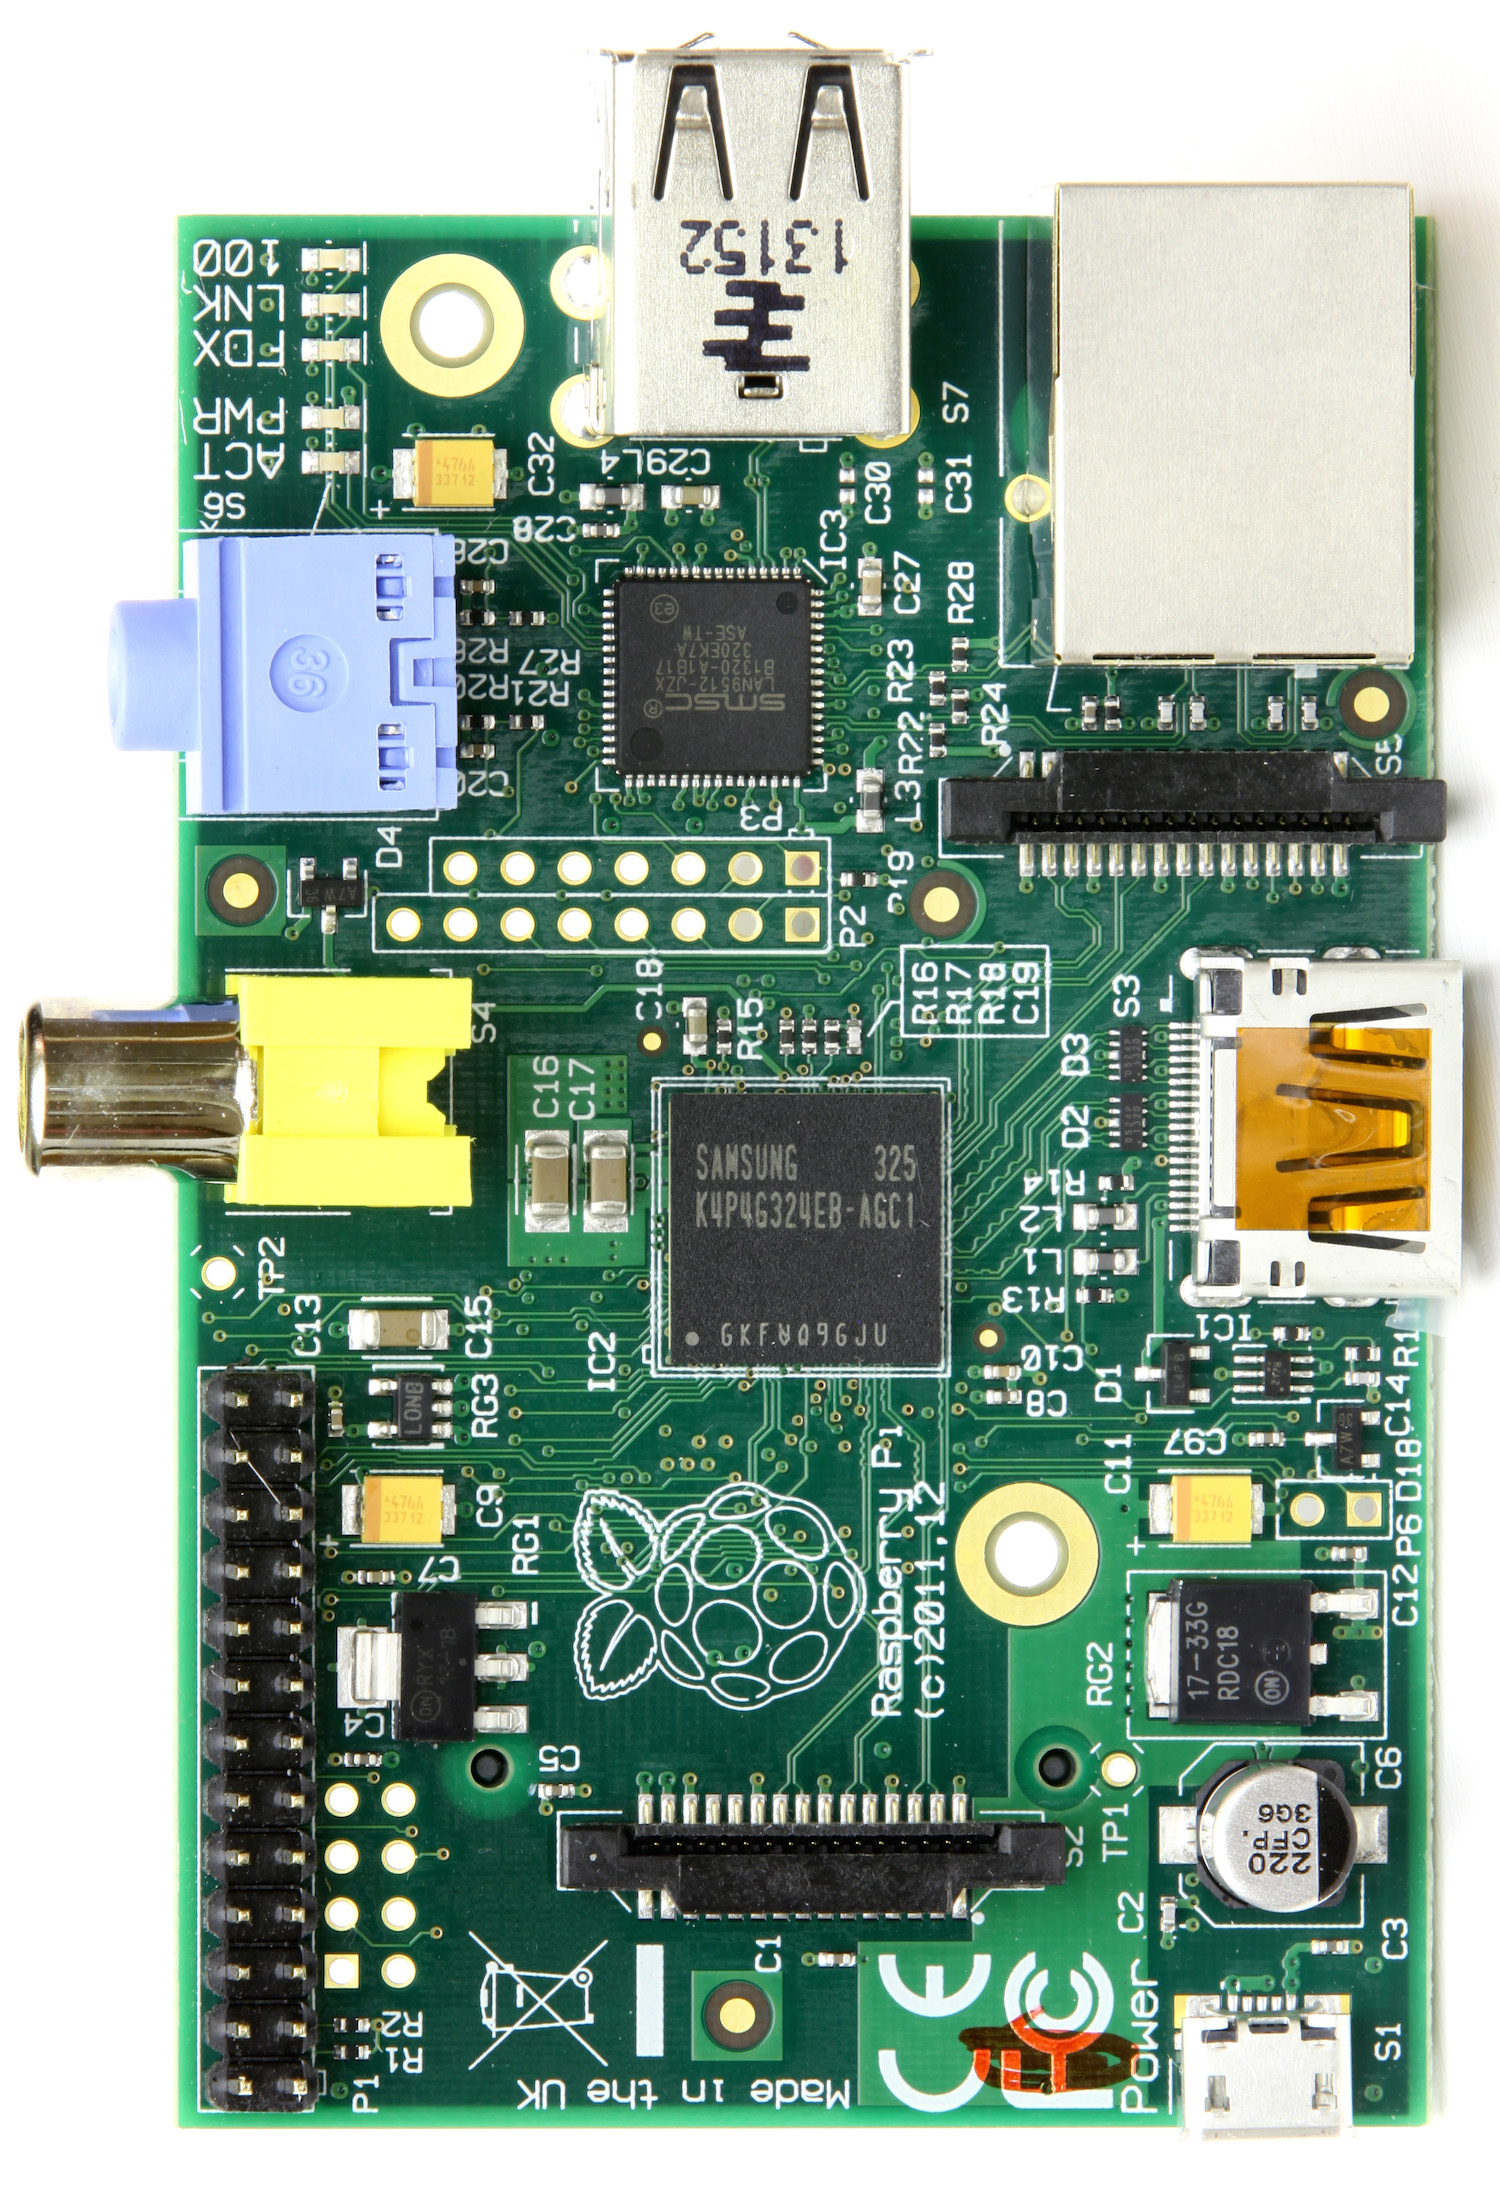
\includegraphics[width=3cm]{img/raspi.png}};
%		\node at (-2.8,-3.3) {
\includegraphics[width=4cm]{img/music.png}};
%		\pause
%		\draw[line width=0.6em,color=blue] (1,1.8) .. controls (1,3) and(4,3) .. (4,1.8);
%		\node[below] at (3.97,2) {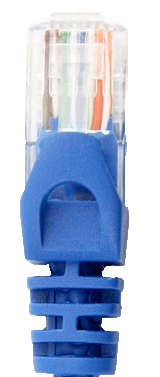
\includegraphics[angle=180,width=0.7cm]{img/plug.png}};
%		\node[below] at (0.97,2) {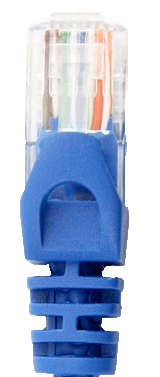
\includegraphics[angle=180,width=0.7cm]{img/plug.png}};
%		%redraw
%		\node at (0,-1.2) {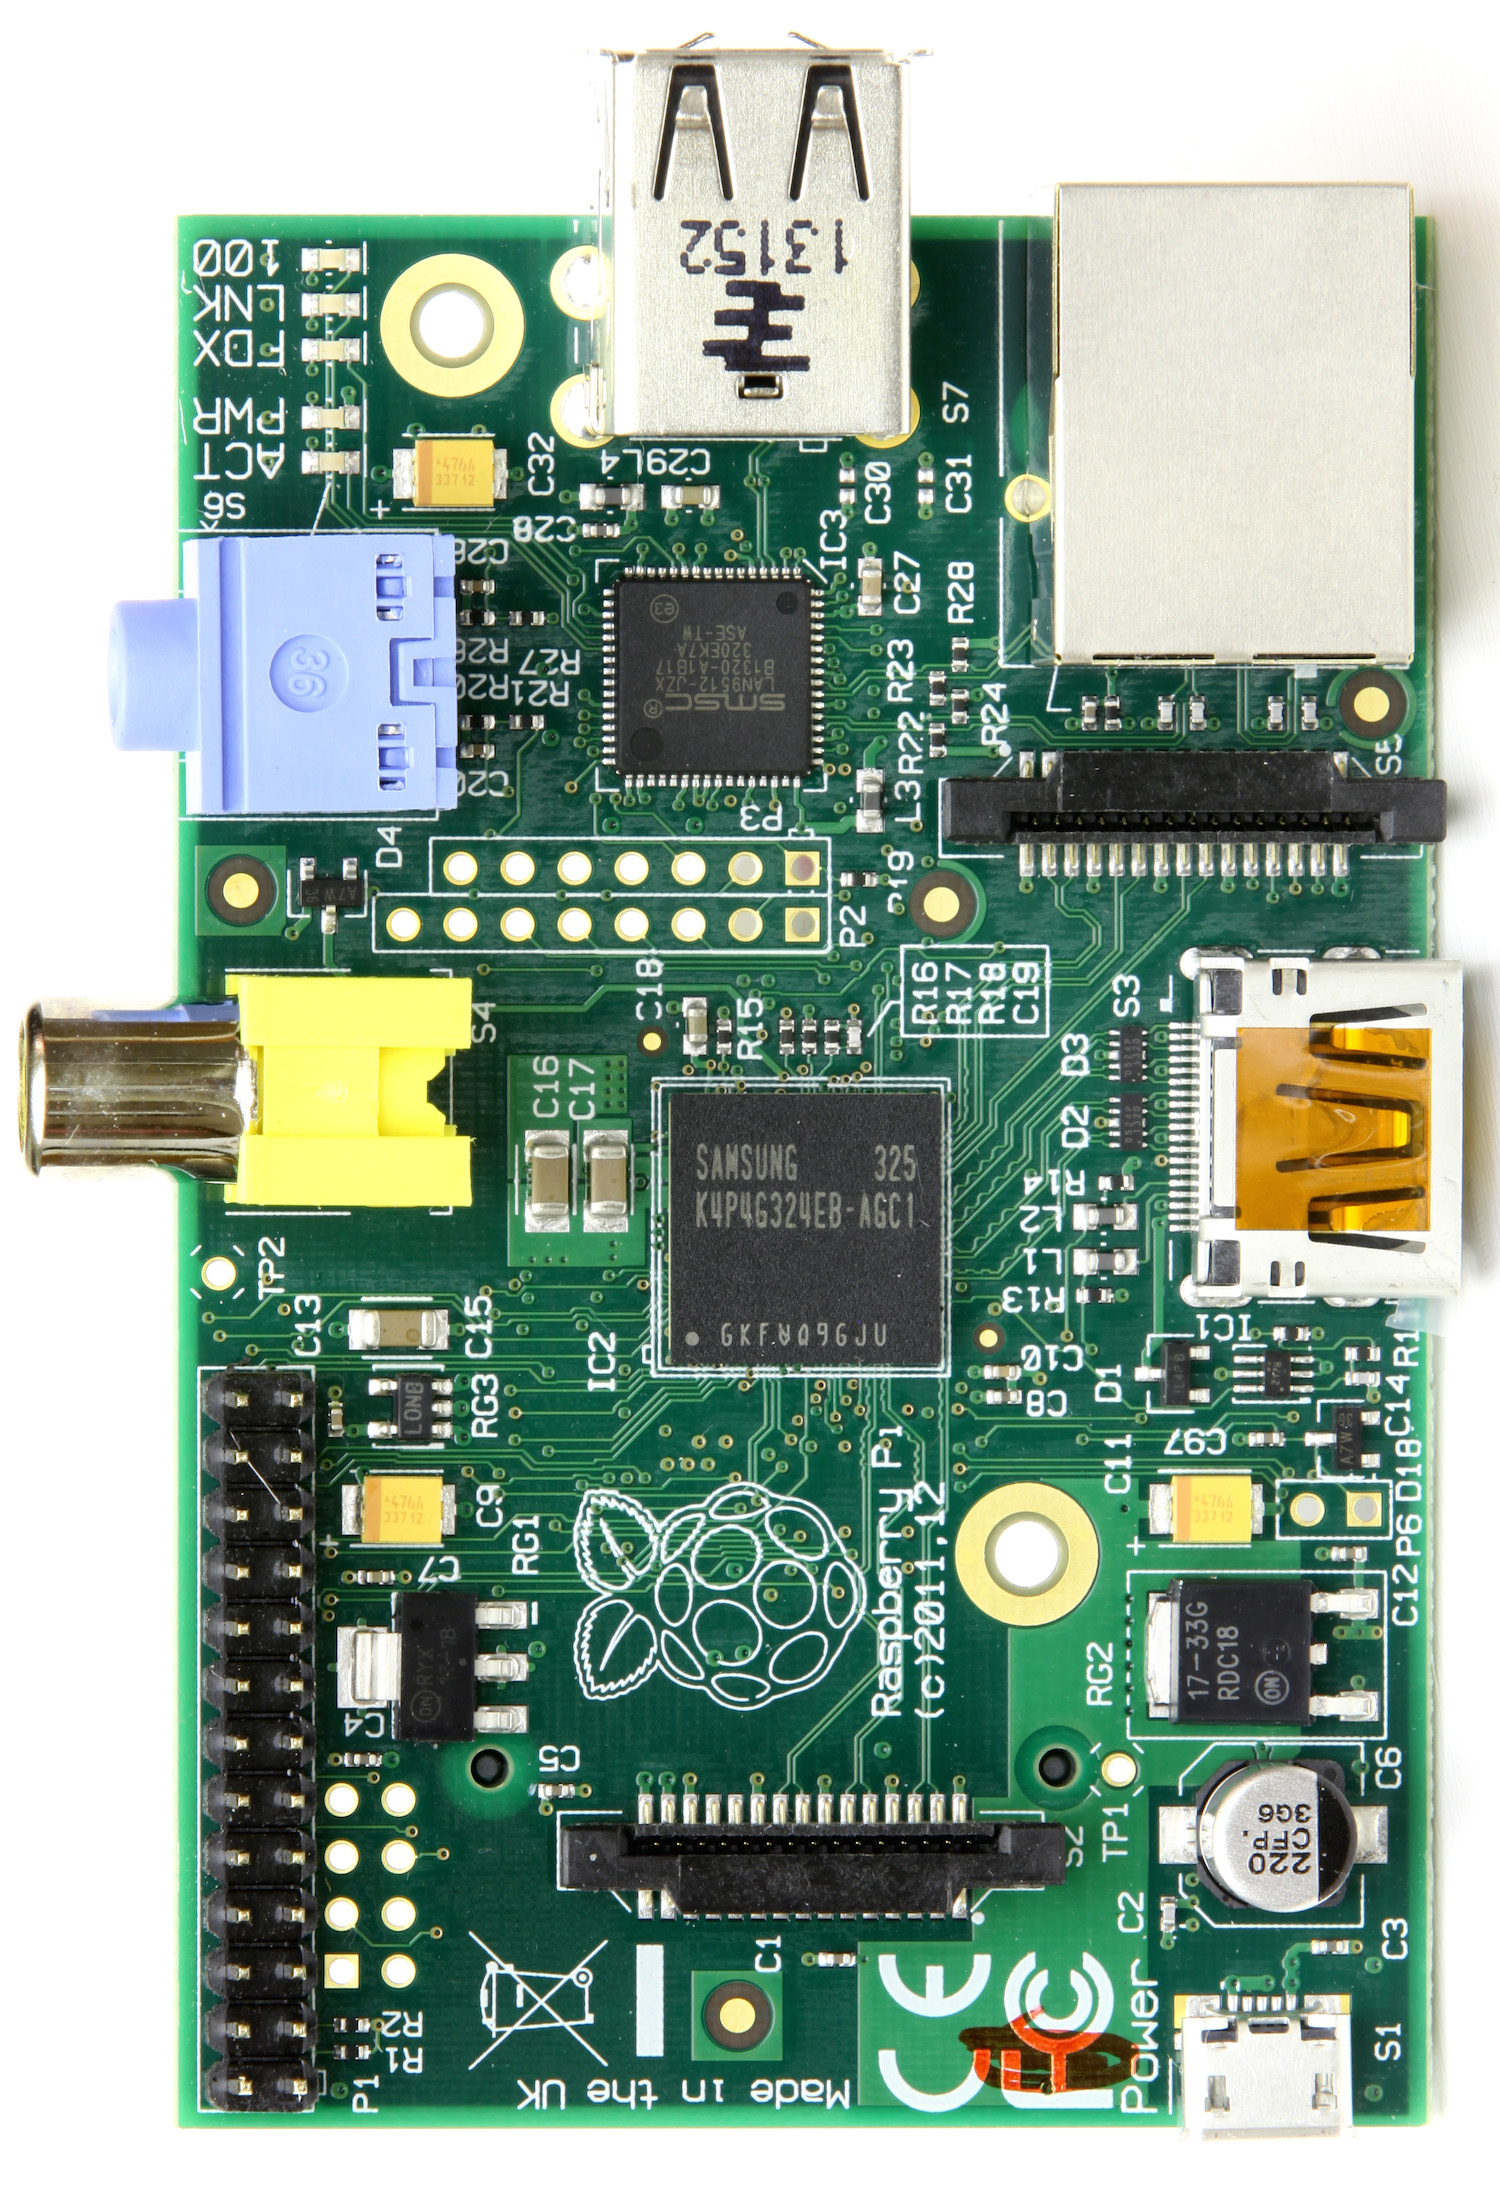
\includegraphics[width=3cm]{img/raspi.png}};
%		\node at (-2.8,-3.3) {
\includegraphics[width=4cm]{img/music.png}};
%		
%		\draw (3,-2) rectangle node{Ethernet} +(2,0.5) 
%			++(0,0.5) rectangle node{IP} +(2,0.5);
%		\pause
%		\draw (3,-1) rectangle node{UDP} +(2,0.5);
%		\pause
%		\draw (3,-0.5) rectangle node{rtpMIDI} +(2,0.5);
%		\pause
%		\fill[white] (2.9,-0.5) rectangle +(2.2,0.6);
%		\draw (3,-0.5) -- +(2,0);
%		\draw (2,-0.5) rectangle node{mDNS} +(2,0.5)
%			++(2,0) rectangle node{rtpMIDI} +(2,0.5);
%	\end{tikzpicture}
%\end{frame}
%\begin{frame}
%	\centering
%	\begin{tikzpicture}
%		\node at (0,-1.2) {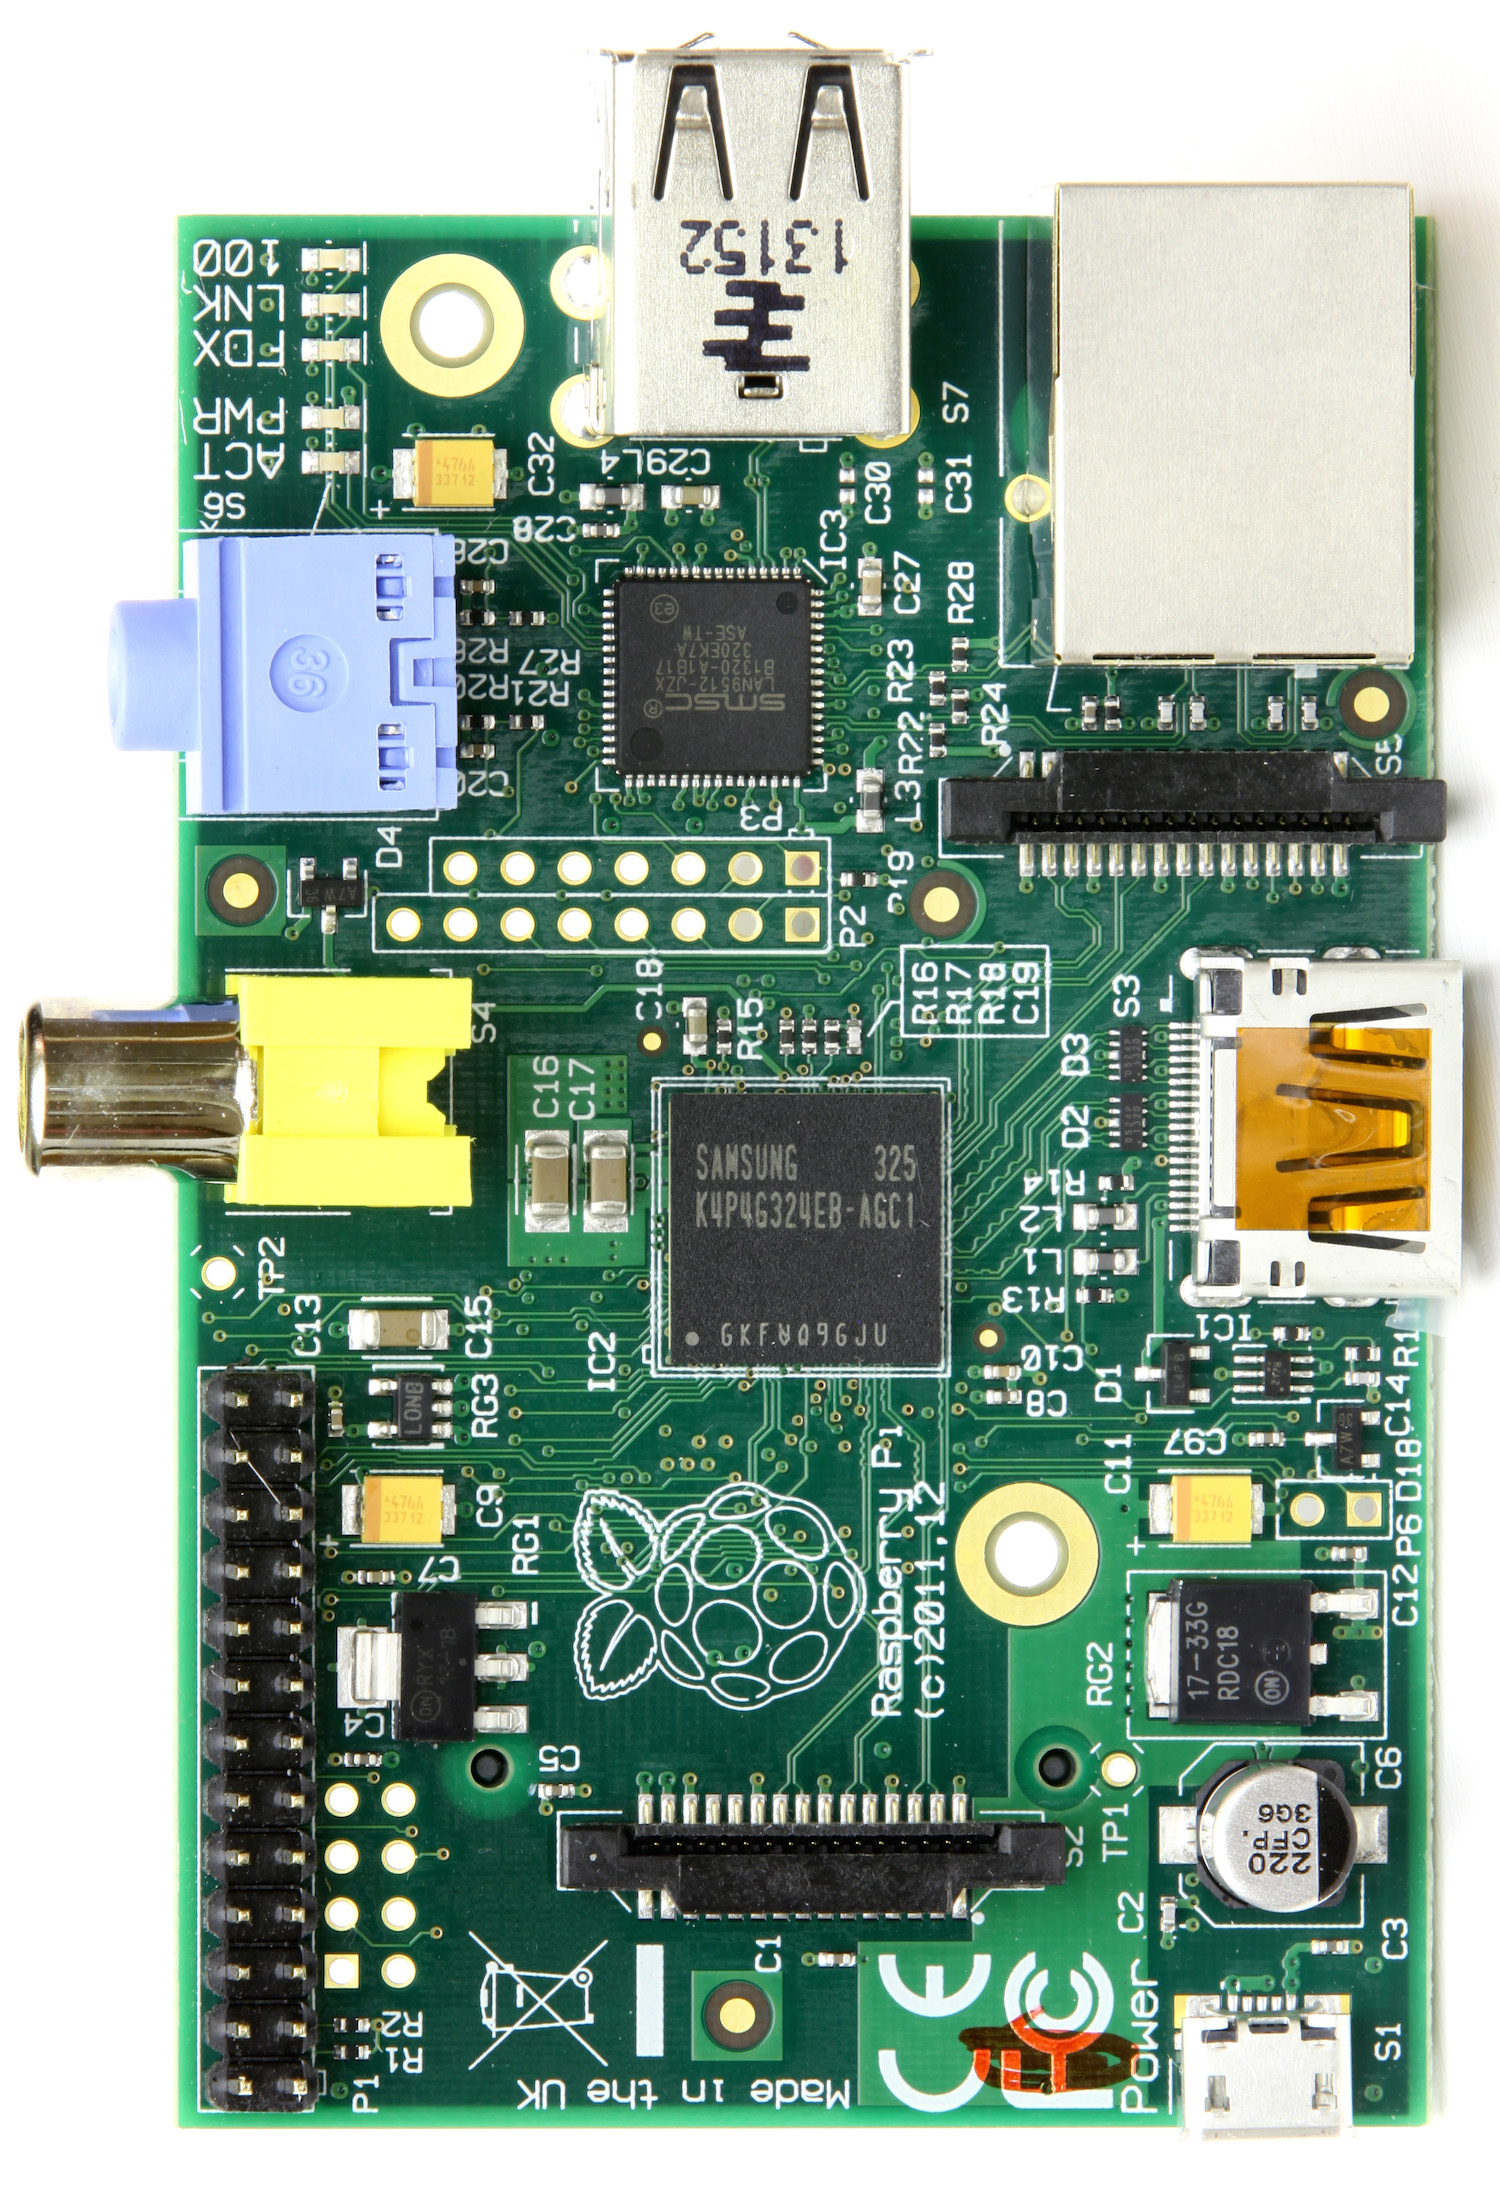
\includegraphics[width=3cm]{img/raspi.png}};
%		\node at (-2.8,-3.3) {
\includegraphics[width=4cm]{img/music.png}};
%		\draw[line width=0.6em,color=blue] (1,1.8) .. controls (1,3) and(4,3) .. (4,1.8);
%		\node[below] at (3.97,2) {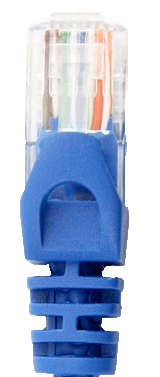
\includegraphics[angle=180,width=0.7cm]{img/plug.png}};
%		\node[below] at (0.97,2) {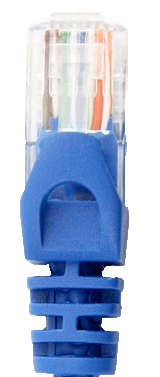
\includegraphics[angle=180,width=0.7cm]{img/plug.png}};
%		%redraw
%		\node at (0,-1.2) {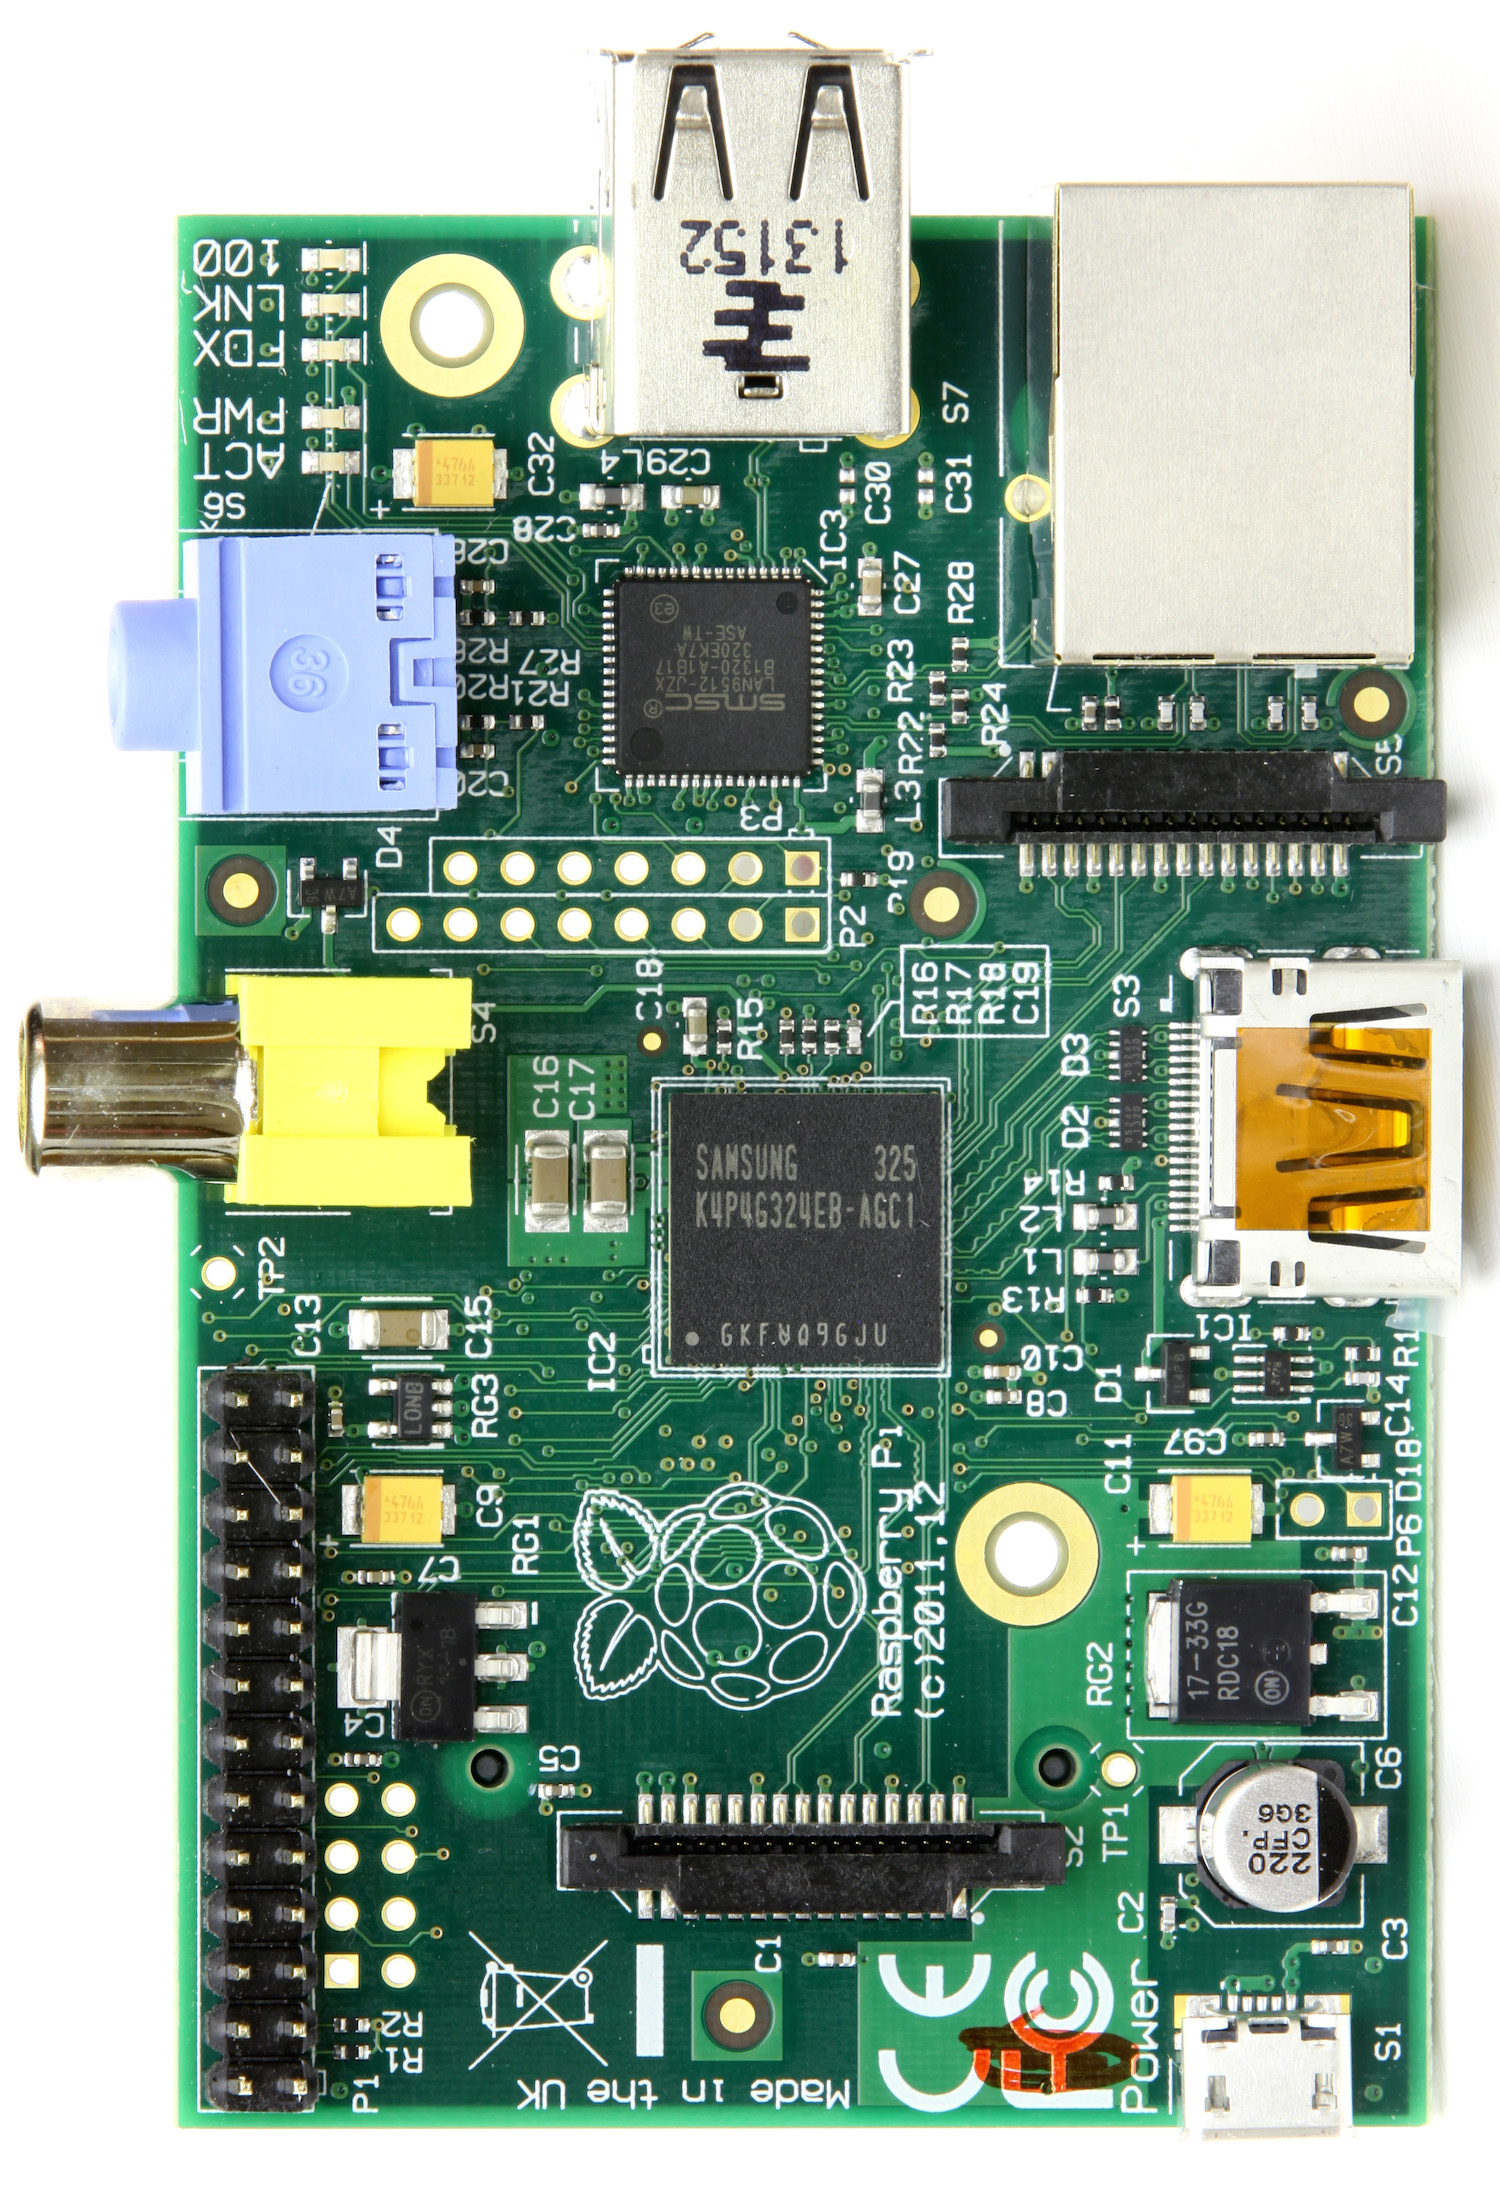
\includegraphics[width=3cm]{img/raspi.png}};
%		\node at (-2.8,-3.3) {
\includegraphics[width=4cm]{img/music.png}};
%		
%		\draw (3,-2.5) rectangle node{Ethernet} +(2,0.5) 
%			++(0,0.5) rectangle node{IP} +(2,0.5);
%		\draw (3,-1.5) rectangle node{UDP} +(2,0.5);
%		\draw (3,-1) rectangle node{SDP} +(2,0.5);
%		\draw (2,-0.5) rectangle node{mDNS} +(2,0.5)
%			++(2,0) rectangle node{rtpMIDI} +(2,0.5);
%	\end{tikzpicture}
%\end{frame}
\begin{frame}
	\centering
	\begin{tikzpicture}
		\node at (0,-1.2) {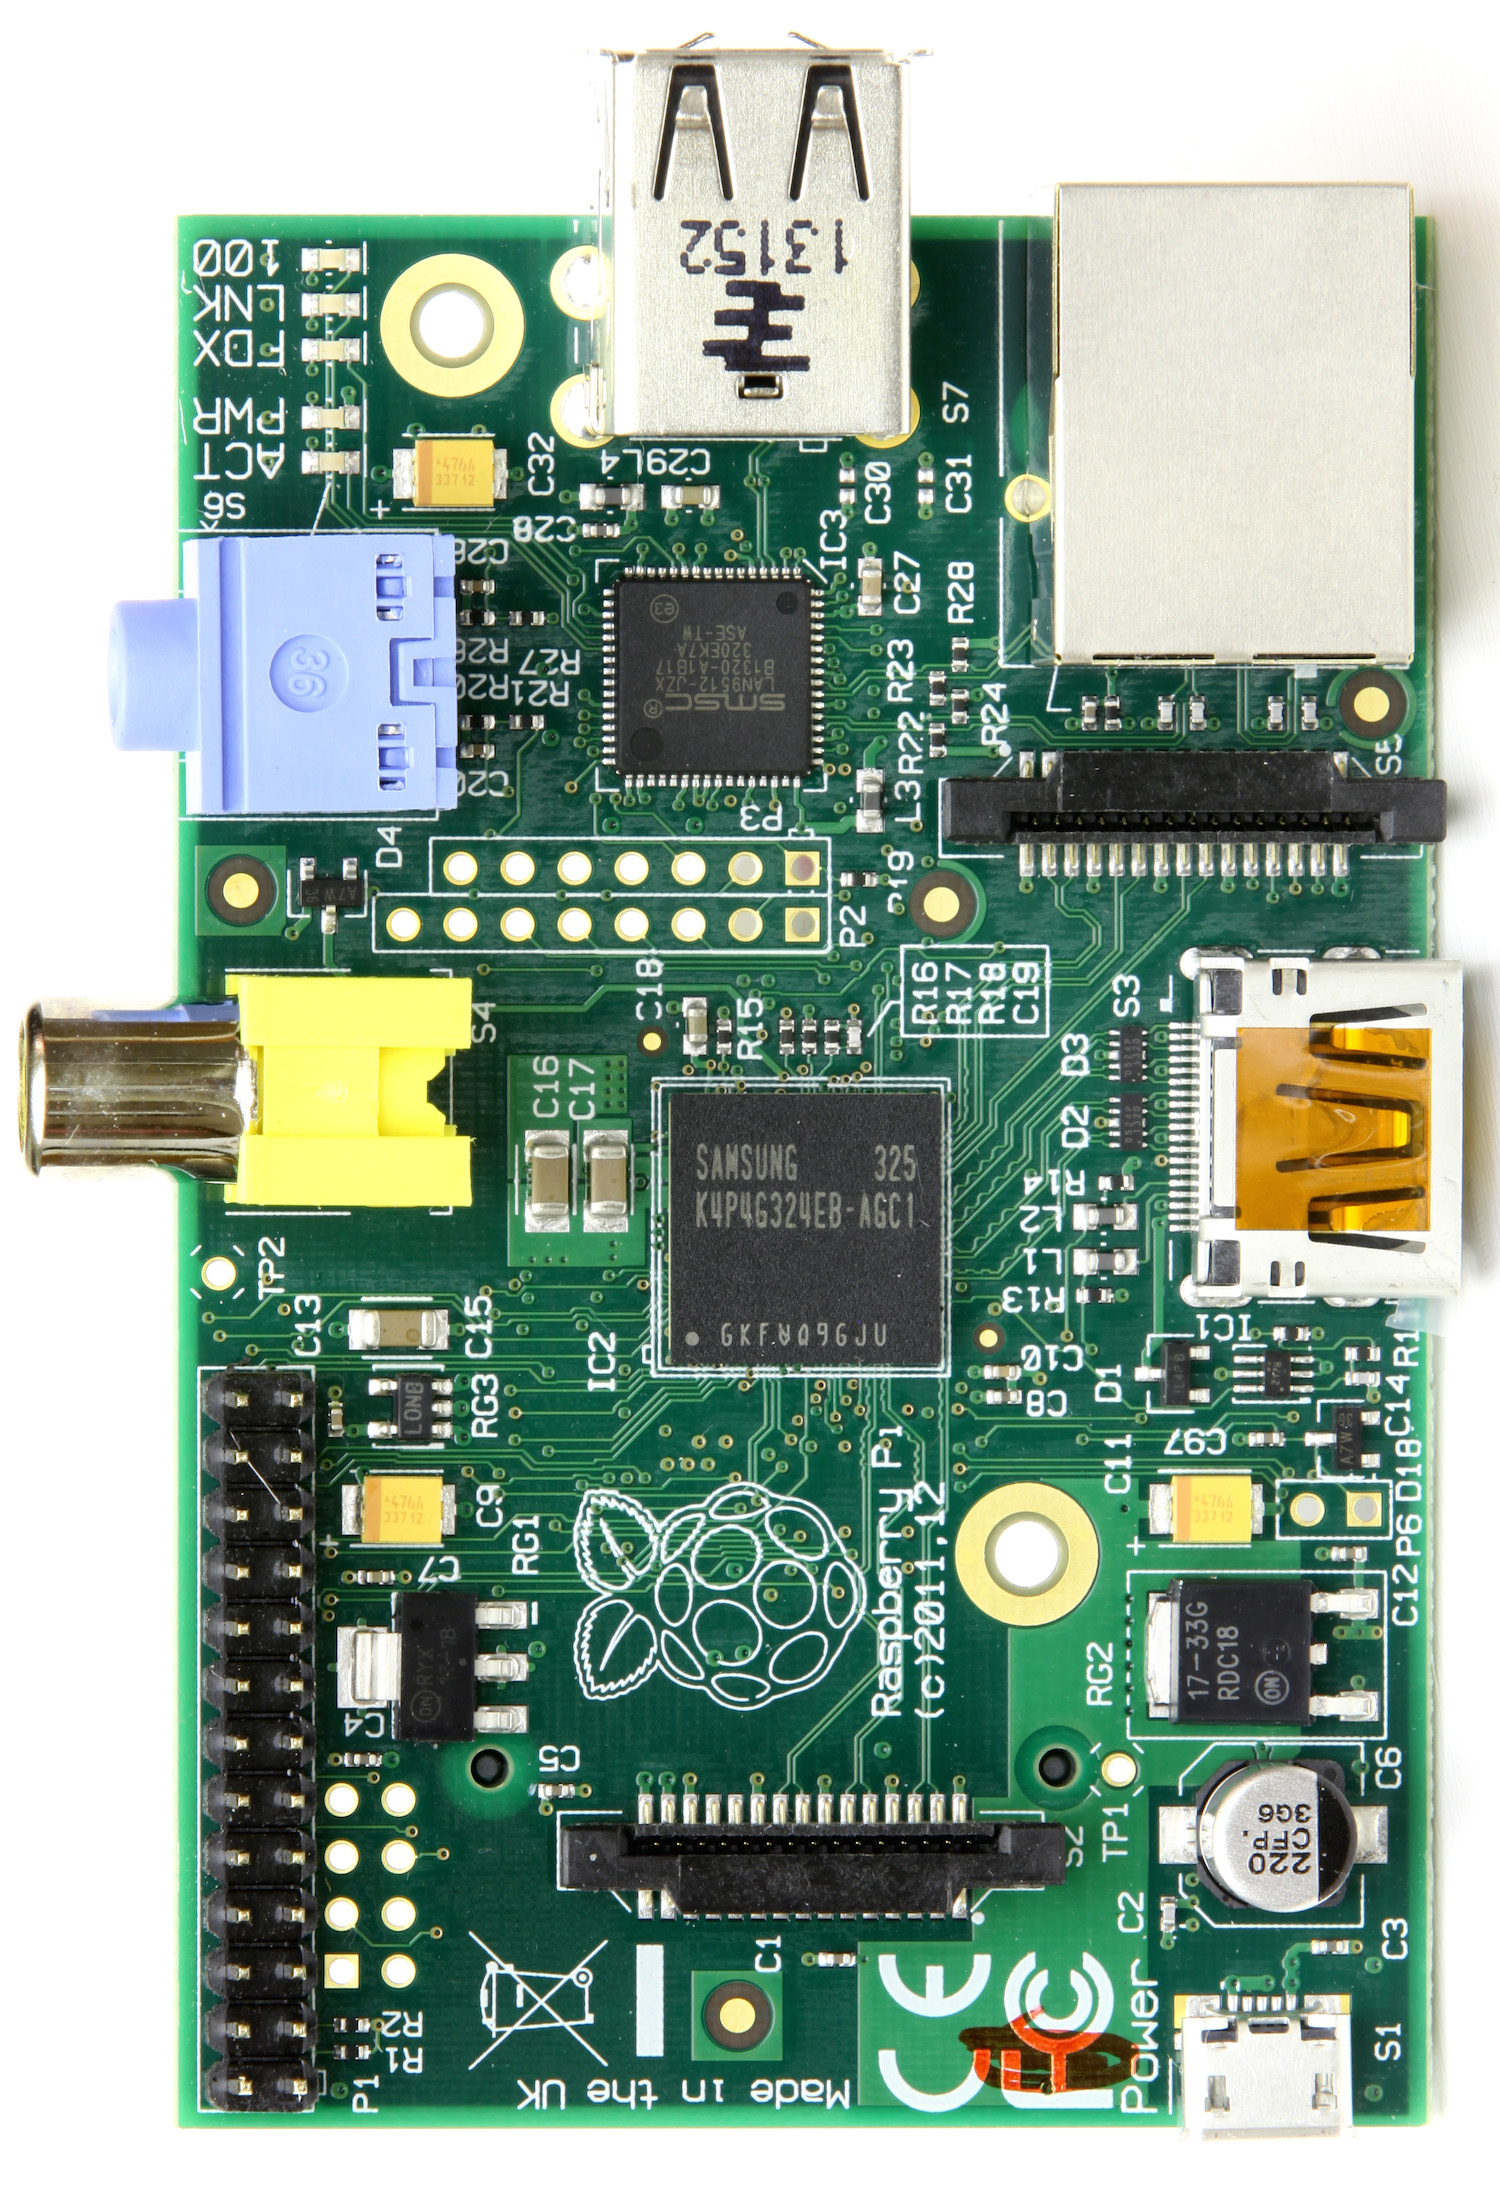
\includegraphics[width=3cm]{img/raspi.png}};
		\node at (-2.8,-3.3) {
\includegraphics[width=4cm]{img/music.png}};
		\pause
		\draw[line width=0.6em,color=blue] (1,1.8) .. controls (1,3) and(4,3) .. (4,1.8);
		\node[below] at (3.97,2) {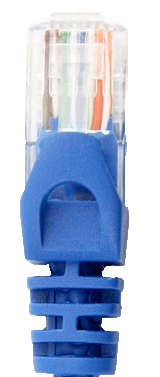
\includegraphics[angle=180,width=0.7cm]{img/plug.png}};
		\node[below] at (0.97,2) {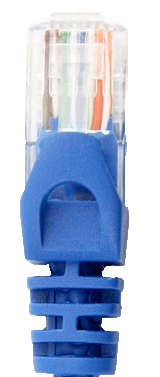
\includegraphics[angle=180,width=0.7cm]{img/plug.png}};
		%redraw
		\node at (0,-1.2) {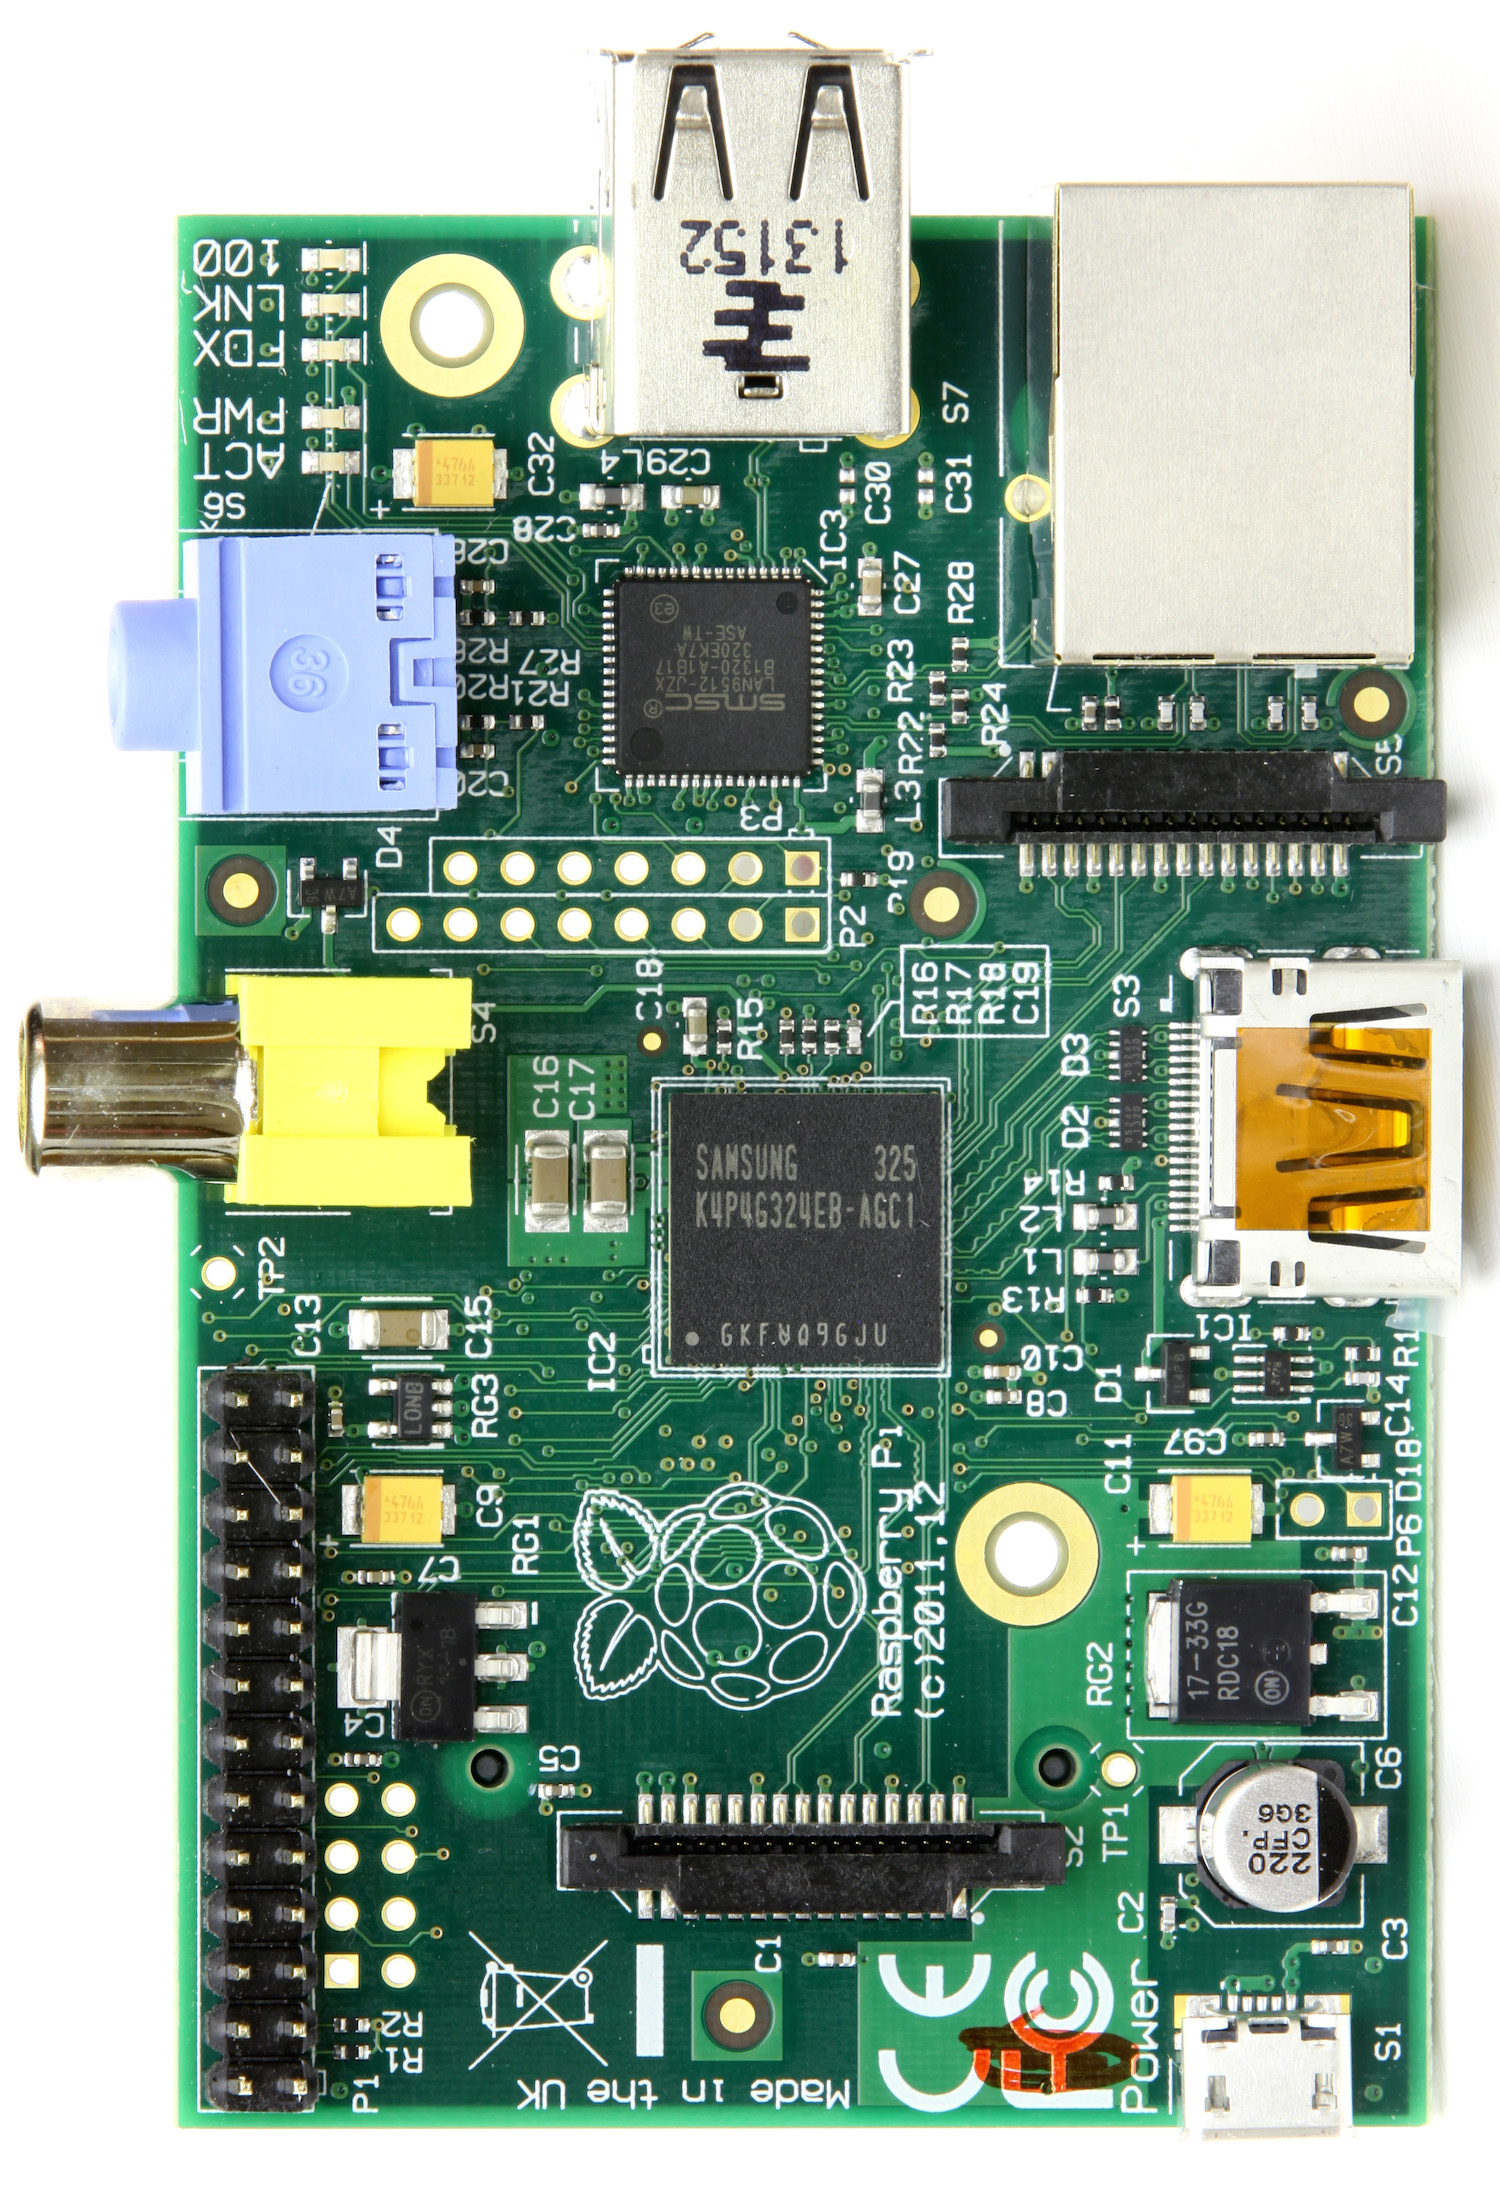
\includegraphics[width=3cm]{img/raspi.png}};
		\node at (-2.8,-3.3) {
\includegraphics[width=4cm]{img/music.png}};
		\pause
		\draw (3,-2) rectangle node{Ethernet} +(2,0.5) 
			++(0,0.5) rectangle node{IP} +(2,0.5);
		\draw (3,-1) rectangle node{UDP} +(2,0.5);
		\draw (2,-0.5) rectangle node{Bonjour} +(2,0.5)
			++(2,0) rectangle node{appleMIDI} +(2,0.5);
	\end{tikzpicture}
\end{frame}
\begin{frame}{rtpMIDI}
	\begin{itemize}
		\item \st{RFC4695} RFC6295 
		\item reference snippets (UCB)
		\pause
		\item closed source
		\begin{itemize}
			\item Core MIDI Framework (OS X)
			\item Windows
			\item nmj (Java)\\$\vdots$
		\end{itemize}
		\pause
		\item open source
		\begin{itemize}
			\item nodejs
			\item midikit (userspace)
		\end{itemize}
	\end{itemize}
\end{frame}

\begin{frame}{kernel driver}
	partial port of midikit to kernel module
	
	features
	\begin{itemize}
		\item AppleMIDI Session Mgnt
		\item synchronization
		\item alsa callbacks for events
		\item RTP-peer management (multiple)
	\end{itemize}
\end{frame}

\begin{frame}{outlook}
	features
	\begin{itemize}
		\item bidirectional (receive RTPMidi)
		\item full MIDI command set
		\item feedback
		\item journal (backward recovery)
	\end{itemize}
	\pause
	analysis
	\begin{itemize}
		\item Jitter
		\item capacity (100 notes/second)
	\end{itemize}
\end{frame}

\begin{frame}
	\centering
	\Huge Demo
\end{frame}
